\documentclass[10pt,UTF8]{ctexart}


\usepackage[margin=2cm,a4paper]{geometry}
%\usepackage[left=0.75in,top=0.6in,right=0.75in,bottom=1.0in,a4paper]{geometry}

\setmainfont{Caladea}
%% 也可以選用其它字庫:
% \setCJKmainfont[%
%   ItalicFont=AR PL KaitiM GB,
%   BoldFont=Noto Sans CJK SC,
% ]{Noto Serif CJK SC}
% \setCJKsansfont{Noto Sans CJK SC}
% \renewcommand{\kaishu}{\CJKfontspec{AR PL KaitiM GB}}

% 繁體中文
\setCJKmainfont[Path=fonts/ ]{NotoSansTC-Medium.otf}

\usepackage{minted}
\usepackage[breaklinks]{hyperref}

% Picture
% 導言區的此三行無變化
\usepackage{graphicx}
\usepackage{float} 
\usepackage{subfigure}
% 以下是新增的自定義格式更改
\usepackage[]{caption2} %新增調用的宏包
\renewcommand{\figurename}{Fig.} %重定義編號前綴詞
\renewcommand{\captionlabeldelim}{.~} %重定義分隔符
 %\roman 是羅馬數字編號,\alph是默認的字母編號,\arabic是阿拉伯數字編號,可按需替換下一行的相應位置
\renewcommand{\thesubfigure}{(\roman{subfigure})}%此外,還可設置圖編號顯示格式,加括號或者不加括號
\makeatletter \renewcommand{\@thesubfigure}{\thesubfigure \space}%子圖編號與名稱的間隔設置
\renewcommand{\p@subfigure}{} \makeatother

% Math
\usepackage {mathtools}
\usepackage{amssymb}

% Code
\usepackage{listings}
\usepackage{xcolor}
\lstset{
    % backgroundcolor=\color{red!50!green!50!blue!50},
    % 程式碼塊背景色為淺灰色
    rulesepcolor= \color{gray}, % 程式碼塊邊框顏色
    breaklines=true,  % 程式碼過長則換行
    numbers=left, % 行號在左側顯示
    numberstyle= \small,% 行號字型
    % eywordstyle= \color{red,% 關鍵字顏色
    commentstyle=\color{gray}, % 註釋顏色
    frame=shadowbox % 用方框框住程式碼塊
    }

\usepackage{hyperref}

\title{計算機視覺作業}
\author{干皓丞,2101212850, 信息工程學院}

\begin{document}
\maketitle


\section{作業目標與章節摘要}

下載運行 YOLOv4 and YOLOv5 的 Python 程式碼,測試 5 幅圖,並於文檔中說明跟之前版本的具體改進和不同。

\section{文章與作業狀況}

作業可以從 GitHub 下的 kancheng/kan-cs-report-in-2021 專案找到,作業程式碼與文件目錄為 kan-cs-report-in-2021/CV/yolo-init。實際執行的環境與實驗設備為 Google 的 Colab 、MacBook Pro (Retina, 15-inch, Mid 2014) 、 Acer Aspire R7 與 HP Victus (Nvidia GeForce RTX 3060)。


\section{YOLO 歷史}

最初由 Joseph Redmon 在 Darknet 中發表,其 YOLO 已經走過了漫長的道路。以下是使 YOLO 的首個版本在 R-CNN 和 DPM 的競爭的過程中脫穎而出的特色:

1. 45 fps 的實時幀處理

2. 減少背景誤報

3. 更高的檢測精度(雖然定位的準確度偏低)

自研究者在 2016 年首次發布以來,該演算法一直在不斷發展。YOLOv2 和 YOLOv3 均由 Joseph Redmon 編寫。在 YOLOv3 之後,出現了新的作者,他們將自己的目標錨定在其他 YOLO 版本中。YOLOv2 在 2017 年發布,由於錨框和分辨率的顯著改進,該版本在 CVPR 2017 上獲得了榮譽獎。YOLOv3 則在 2018 年版本對邊界框預測和與骨幹網絡層的連接有一個額外的客觀性分數。由於能夠在三個不同的粒度級別運行預測,它還提高了對微小對象的性能。而 YOLOv4 於 2020 年 4 月發布的論文成為第一篇非 Joseph Redmon 撰寫的論文。在這裡由 Alexey Bochkovski 介紹了新穎的改進,包括思維激活、改進的特徵聚合等。

最後則是最近期的 YOLOv5,則是由 Glenn Jocher 在 2020 年 6 月的版本中繼續進行進一步改進,其重點放在架構本身,整體用在 Pytorch 上,但他們的重心放在 YOLOv3 的移植跟 YOLOv5 的發展。

而 YOLOv4 和 YOLOv5 之間的性能差異則有 Joseph Nelson, Jacob Solawetz 兩位於 2020 年 1 月 10 號發布的技術文章中有詳細說明,該文章為 'YOLOv5 is Here: State-of-the-Art Object Detection at 140 FPS',而更詳細的測試則於兩天後 2020 年 1 月 12 號發佈名為 'YOLOv5 is Here: State-of-the-Art Object Detection at 140 FPS'。詳細的作業閱讀紀錄連結可以於 init.md 中找到,而當中關鍵的原文摘要如下,同時進行原文翻譯。

"Running a Tesla P100, we saw inference times up to 0.007 seconds per image, meaning 140 frames per second (FPS)! By contrast, YOLO v4 achieved 50 FPS after having been converted to the same Ultralytics PyTorch library."

「在運行 Tesla P100,我們看到每張圖像的推理時間高達 0.007 秒,這意味著每秒 140 幀 (FPS)!相比之下,YOLOv4 在轉換為相同的 Ultralytics PyTorch 庫後達到了 50 FPS。」

"YOLO v5 is small. Specifically, a weights file for YOLO v5 is 27 megabytes. Our weights file for YOLO v4 (with Darknet architecture) is 244 megabytes. YOLO v5 is nearly 90 percent smaller than YOLO v4."

「YOLOv5 比較小。具體來說,YOLOv5 的權重文件為 27 兆字節。我們的 YOLOv4(具有暗網架構)的權重文件為 244 兆字節。YOLOv5 比 YOLOv4 小了近 90 \% 。這意味著 YOLOv5 可以更輕鬆地部署到嵌入式設備。」

"YOLOv5 achieves 140 frames per second in batch, which the YOLOv5 implementation tested utilizes by default. When batch size is set to 1, YOLOv4 achieves 30 FPS while YOLOv5 outputs 10 FPS."

「YOLOv5 達到每秒 140 幀在批次,其 YOLOv5 執行默認測試利用。當批量大小設置為 1 時,YOLOv4 達到 30FPS,而 YOLOv5 輸出 10 FPS。」


\begin{figure}[H]
\centering 
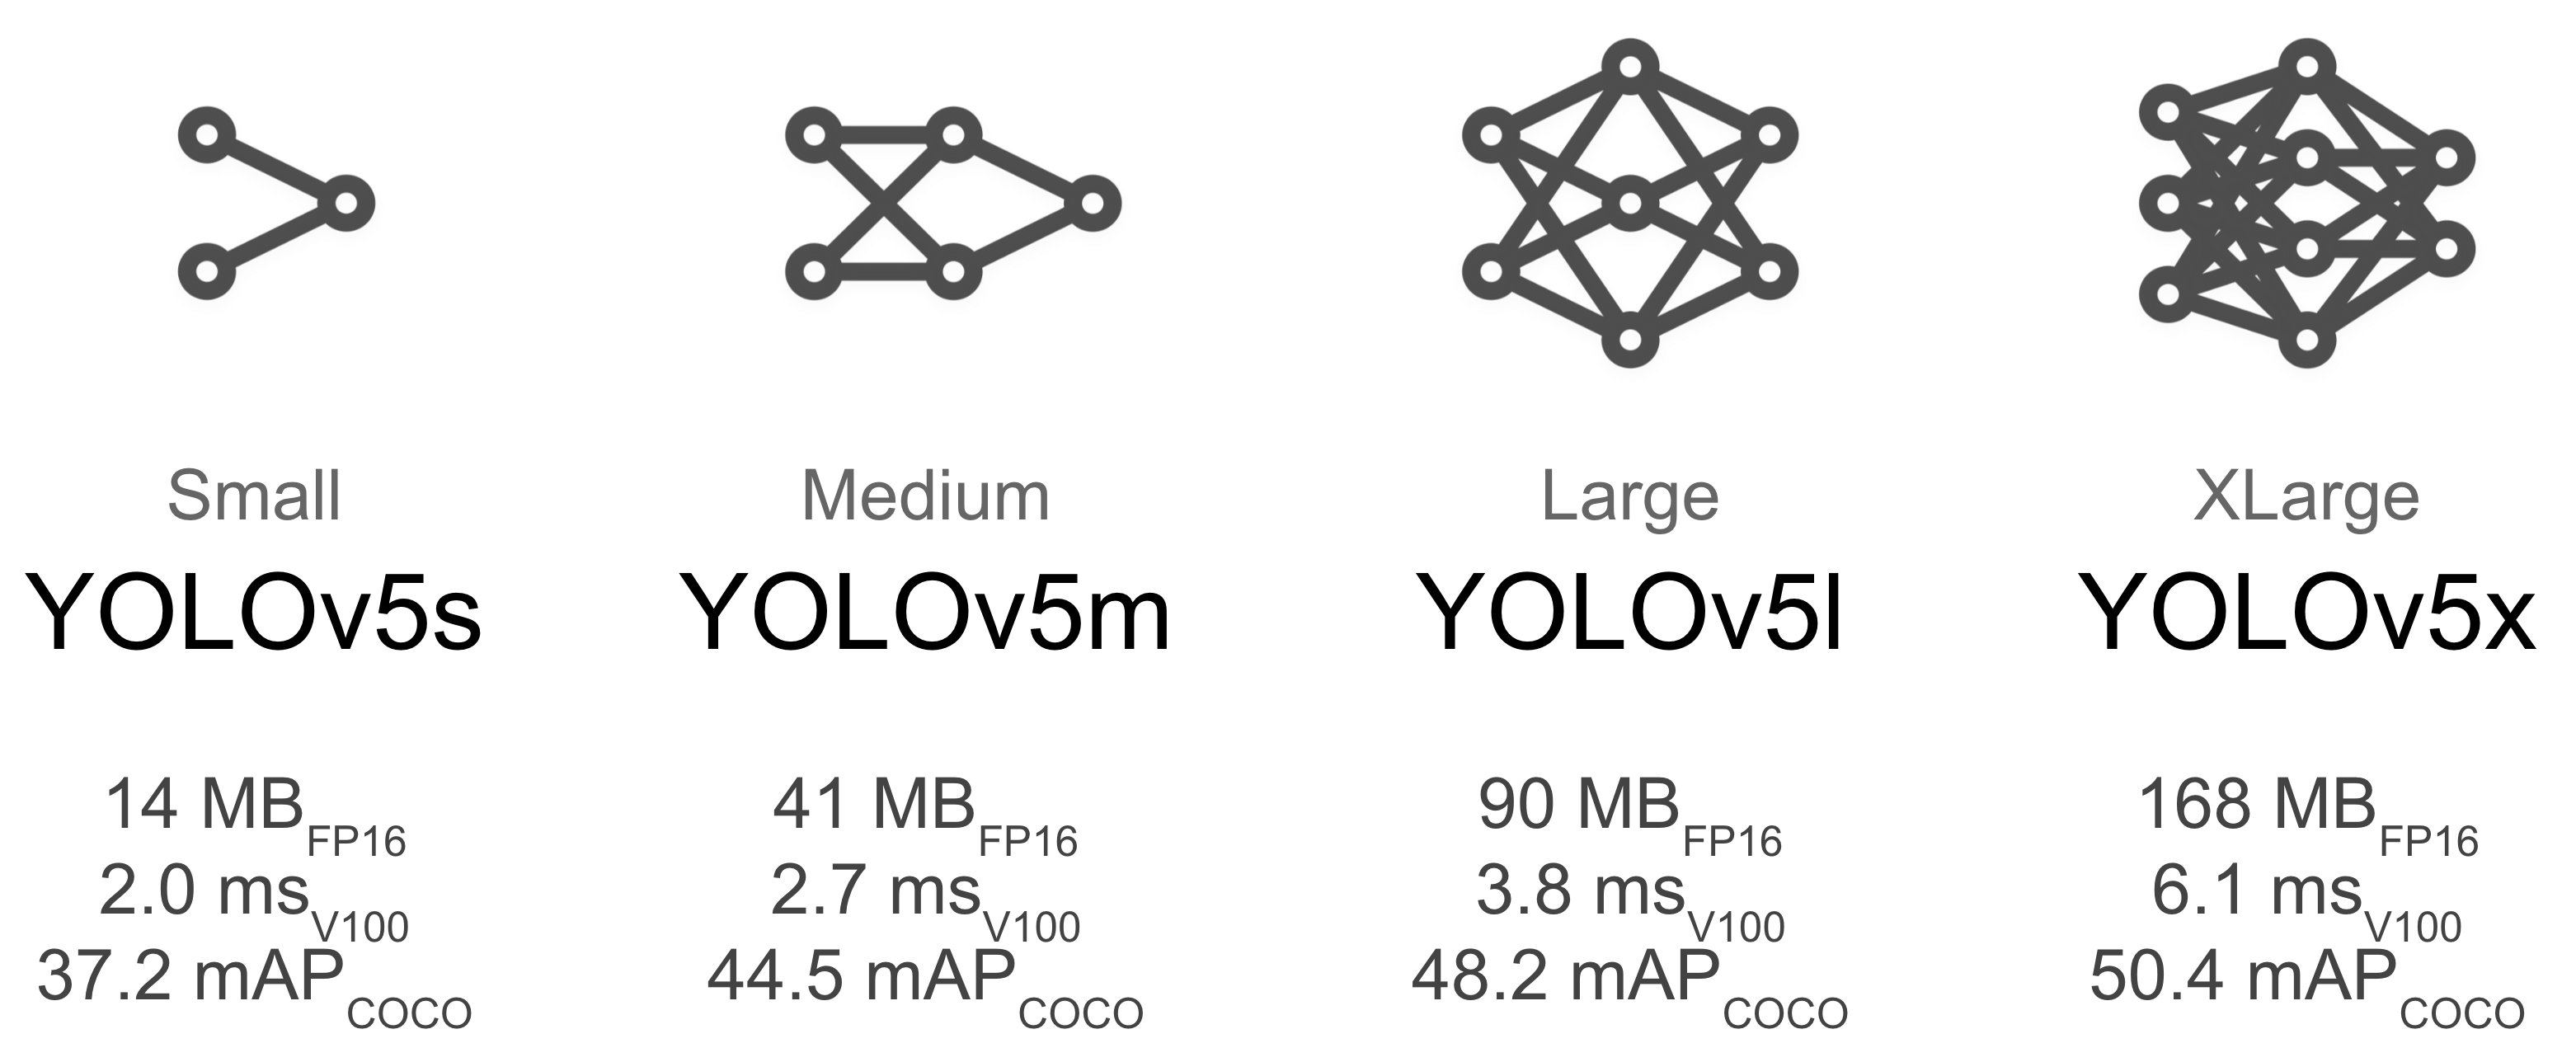
\includegraphics[width=0.80\textwidth]{d1.png} 
\caption{YOLOv5 模型說明}
\label{Test}
\end{figure}

\begin{figure}[H]
\centering 
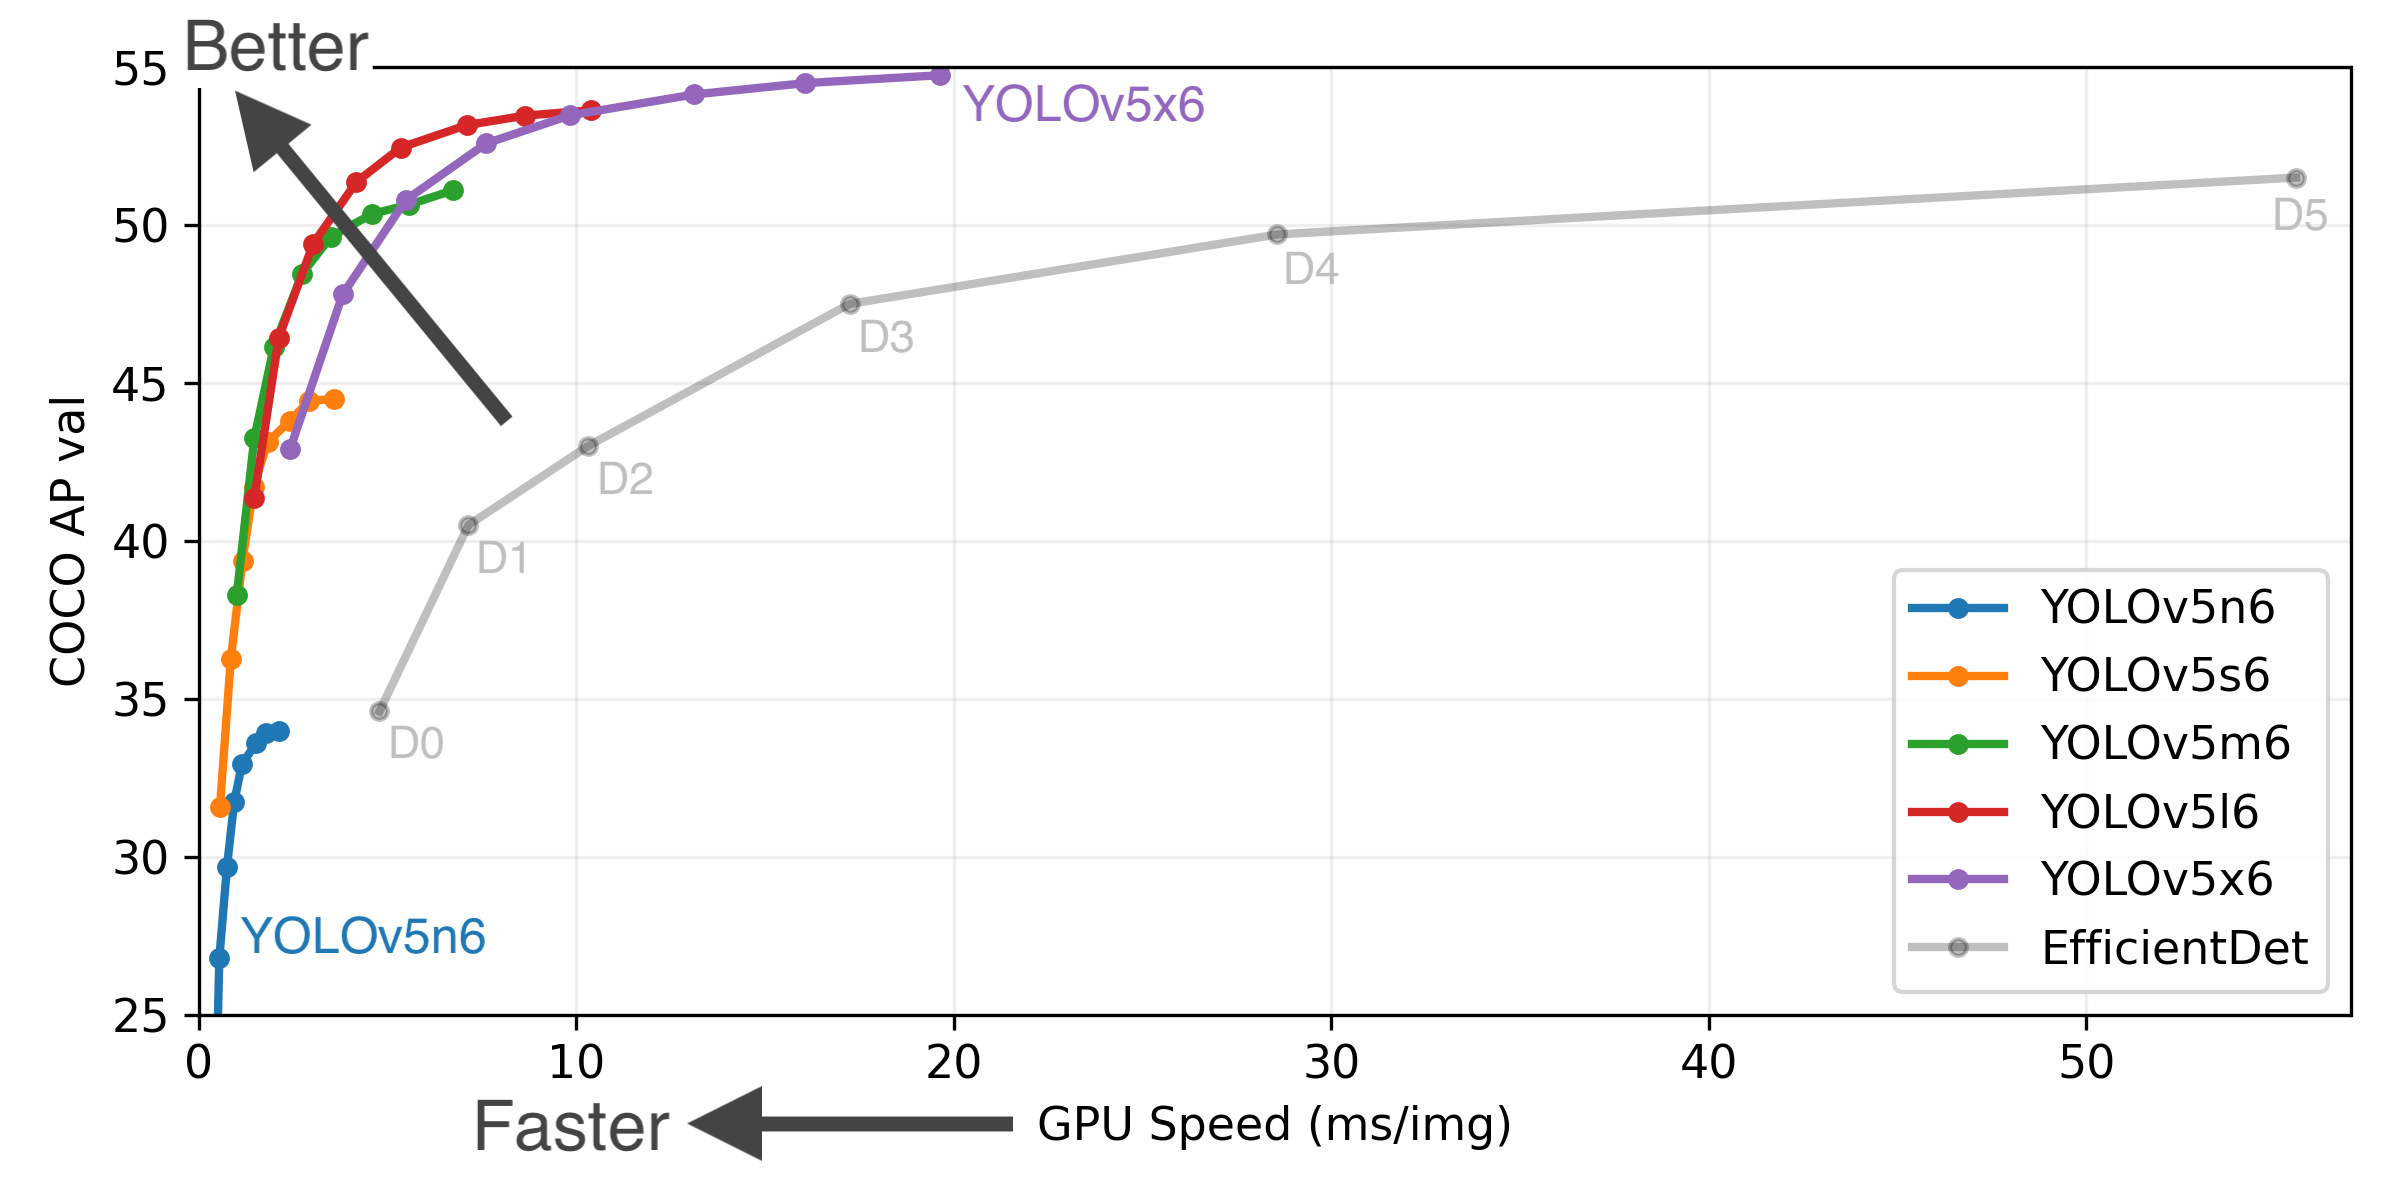
\includegraphics[width=0.90\textwidth]{d2.png} 
\caption{效能指標}
\label{Test}
\end{figure}

\newpage

\section{Experiment with YOLOv3 and YOLOv4 on TensorFlow}

可以從專案中 code 目錄下,找到 tranleanh/darkeras-yolov4 專案的 YOLOv3 和 YOLOv4 的 TensorFlow 版本。其檔案為 darkeras-yolov3.ipynb 和 darkeras-yolov4.ipynb 。還原環境與模型後可以得到指定的結果。

\begin{figure}[H]
\centering 
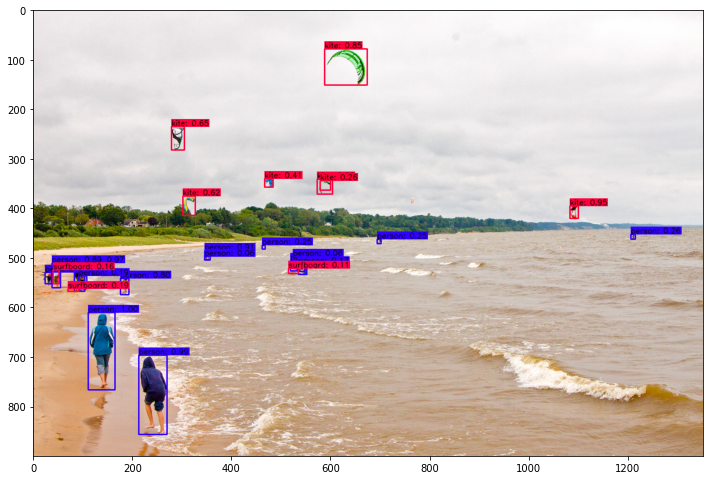
\includegraphics[width=0.90\textwidth]{dyolo3.png} 
\caption{YOLOv3 結果呈現}
\label{Test}
\end{figure}

\begin{figure}[H]
\centering 
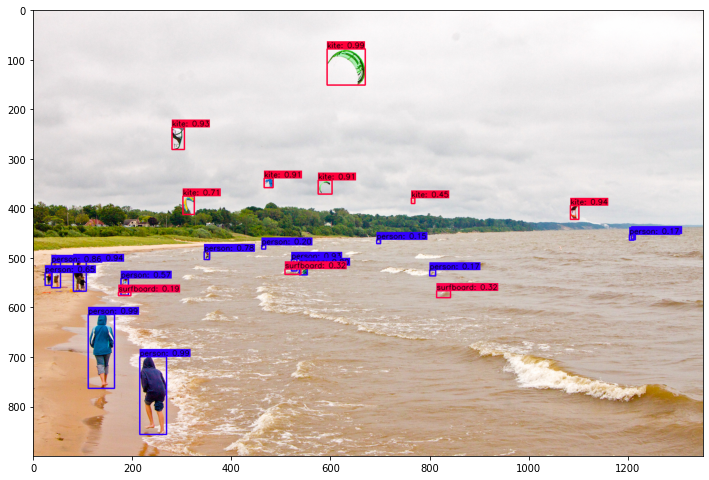
\includegraphics[width=0.90\textwidth]{dyolo4.png} 
\caption{YOLOv4 結果呈現}
\label{Test}
\end{figure}

\newpage


\section{Experiment with YOLOv5 on Pytorch}

YOLOv5 則分為兩大部分,其一為 Pytorch 官方的 Google 的 Colab 官方案例,另外為自己還原 ultralytics/yolov5 官方專案後,使用自己資料執行的結果,誠然官方也有給 Docker 的環境方案,但由於設備、環境跟時間因素,經研究後放棄。其指令說明如下 :

\begin{lstlisting}[language={python}]
# 建立虛擬環境
conda create -n test-volo python=3.8

# 進入虛擬環境
conda activate test-volo

# 官方專案
git clone https://github.com/ultralytics/yolov5.git

# Pytorch
conda install pytorch torchvision torchaudio cudatoolkit=11.3 -c pytorch

# 官方套件指定安裝
pip install -r requirements.txt

# 中國大陸地區網路環境建議使用
pip install -r requirements.txt -i https://pypi.tuna.tsinghua.edu.cn/simple

# 模型
python detect.py --weights yolov5s.pt

python detect.py --weights yolov5m.pt

python detect.py --weights yolov5s6.pt

python detect.py --weights yolov5m6.pt

# 測試
python detect.py --source data/images --weights yolov5s.pt --conf 0.25
\end{lstlisting}

其實際過程與截圖說明如下。

\begin{figure}[H]
\centering 
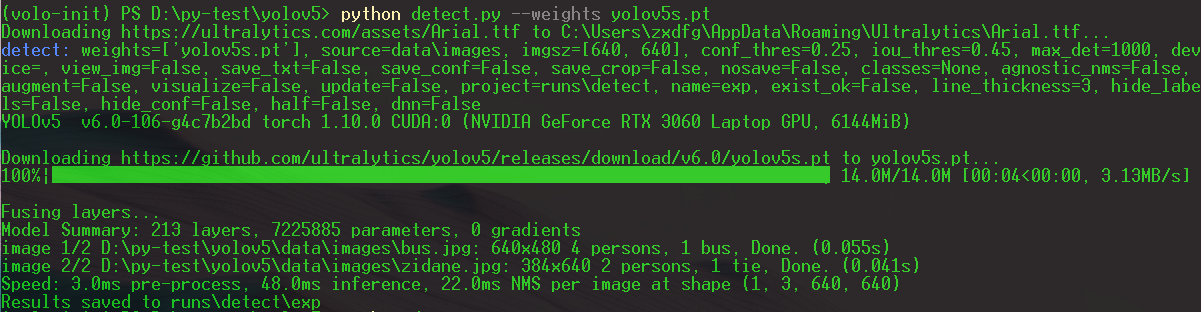
\includegraphics[width=0.90\textwidth]{n1.png} 
\caption{Weights yolov5s.pt}
\label{Test}
\end{figure}

\begin{figure}[H]
\centering 
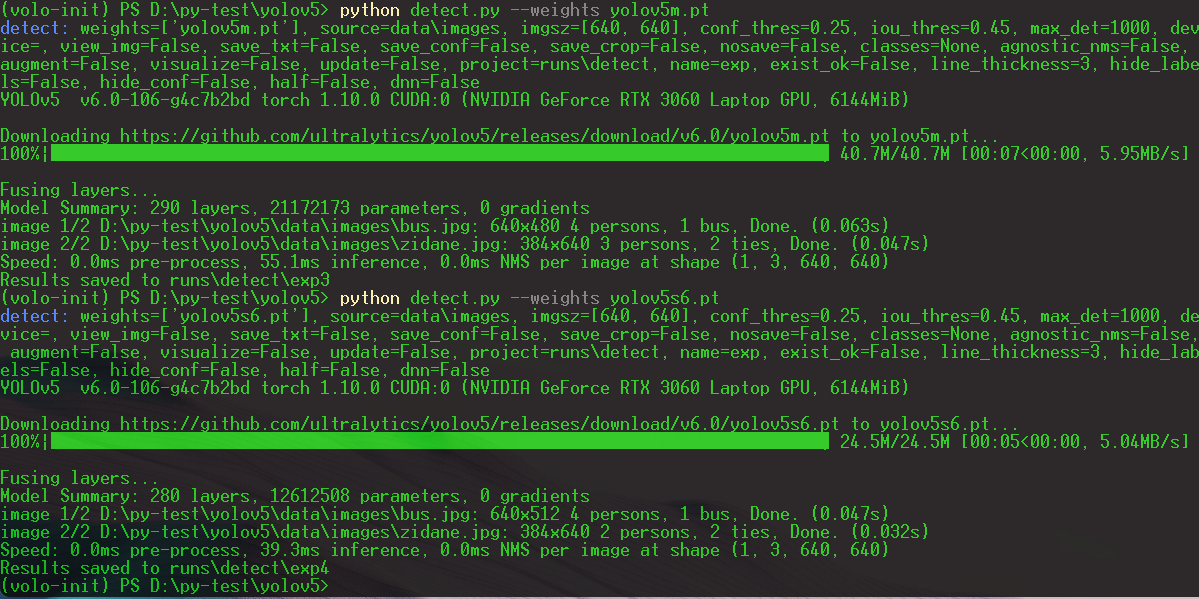
\includegraphics[width=0.90\textwidth]{n2.png} 
\caption{Weights yolov5m.pt and yolov5s6.pt}
\label{Test}
\end{figure}

\begin{figure}[H]
\centering 
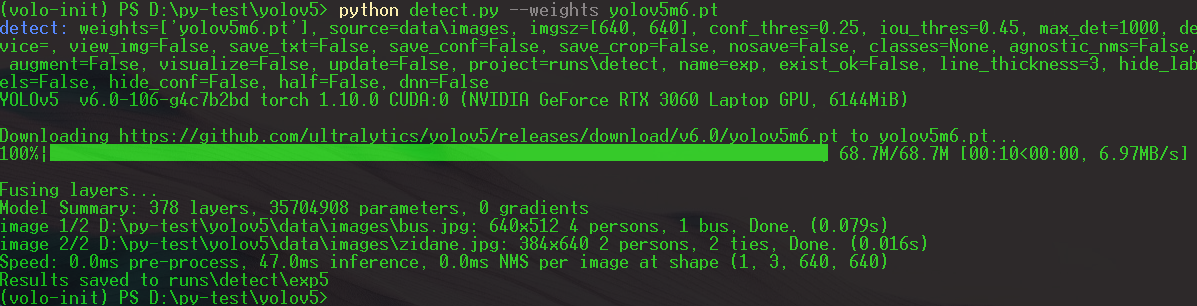
\includegraphics[width=0.90\textwidth]{n3.png} 
\caption{Weights yolov5m6.pt}
\label{Test}
\end{figure}

接下來進行第一輪測試的實驗從官方與自己相簿跟新聞的圖做為測試資料。第一輪與第二輪分別用的是 yolov5s.pt 與 yolov5m.pt,其過程截圖如下所示。

\begin{figure}[H]
\centering 
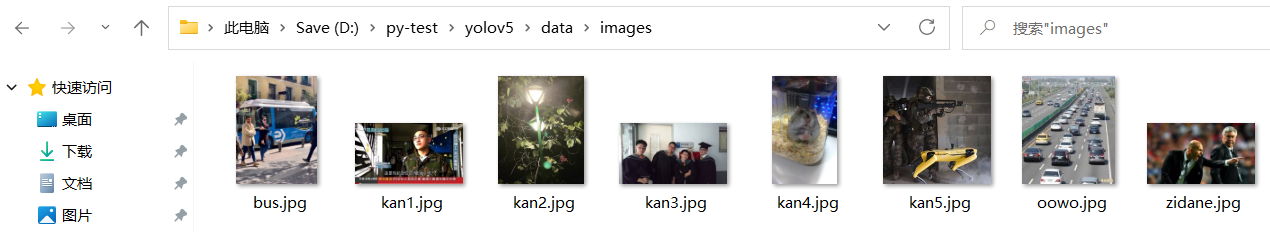
\includegraphics[width=0.90\textwidth]{n4.png} 
\caption{第一輪測試資料}
\label{Test}
\end{figure}

\begin{figure}[H]
\centering 
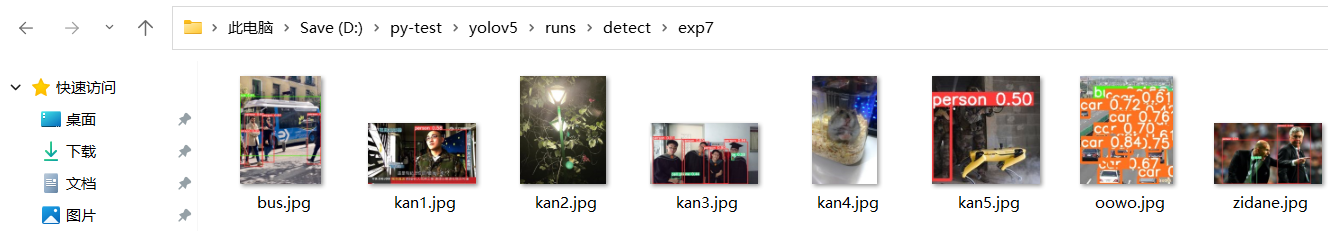
\includegraphics[width=0.90\textwidth]{n5.png} 
\caption{第一輪測試結果}
\label{Test}
\end{figure}

\begin{figure}[H]
\centering 
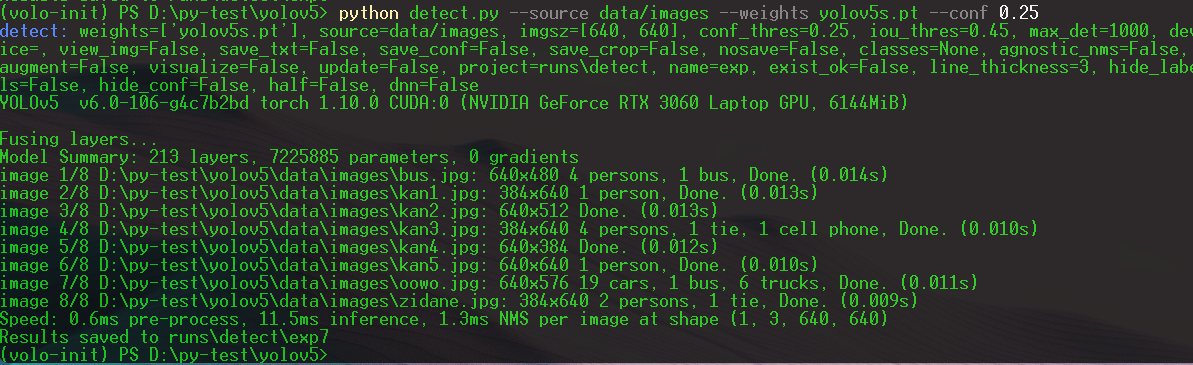
\includegraphics[width=0.90\textwidth]{n6.png} 
\caption{第一輪測試狀況}
\label{Test}
\end{figure}

\begin{figure}[H]
\centering 
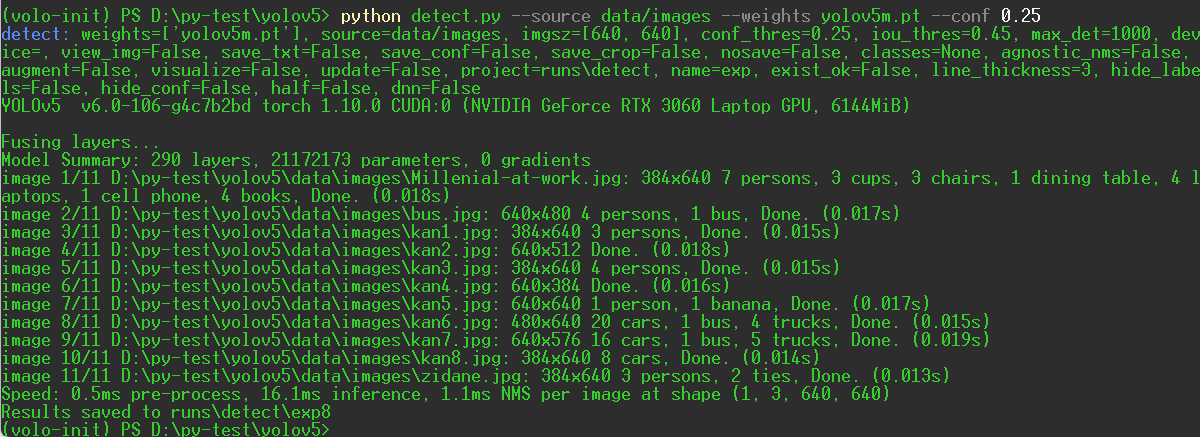
\includegraphics[width=0.90\textwidth]{n7.png} 
\caption{第二輪測試截圖}
\label{Test}
\end{figure}

\newpage

接下來列出原始資料進行說明,同時說明出處,過程中發現倉鼠照片跟北大深研院的路燈照片並沒有正確顯示。當中官方測試圖有三張,交通新聞有三張,人工智慧與機器人新聞一張,軍事新聞一張,生活照一張。

%\begin{figure}[H]
%\centering  %圖片全局居中
%\subfigure[Sigmoid 函數]{
%\label{Fig.sub.1}
%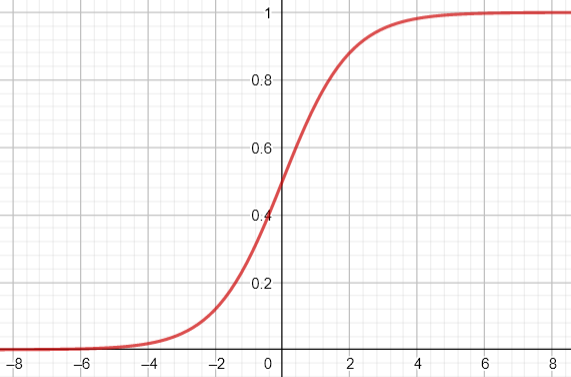
\includegraphics[width=0.45\textwidth]{mp1.png}}
%\subfigure[Sigmoid 函數求導與原函數對比]{
%\label{Fig.sub.2}
%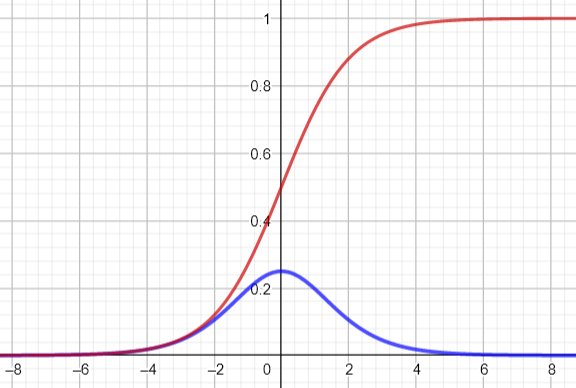
\includegraphics[width=0.45\textwidth]{mp2.png}}
%\caption{Sigmoid函數狀態}
%\label{Fig.main}
%\end{figure}

\begin{figure}[H]
\centering  %圖片全局居中
\subfigure[測試 - 官方]{
\label{Fig.sub.1}
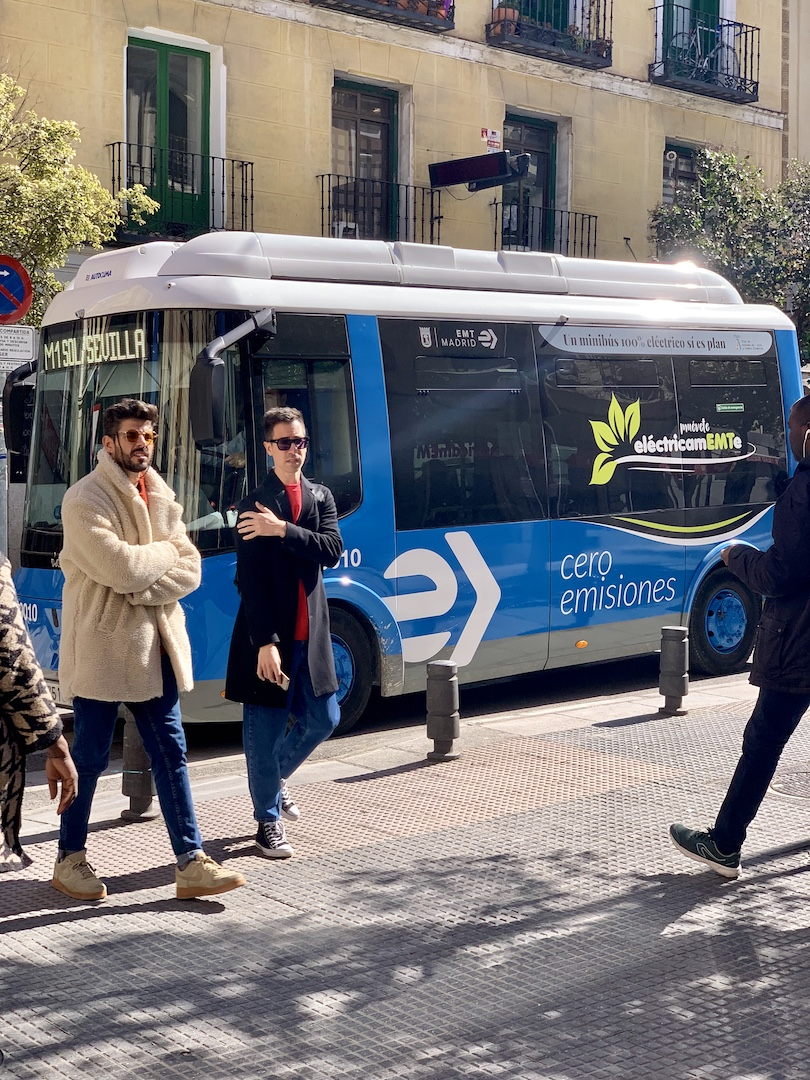
\includegraphics[width=0.3\textwidth]{r1.jpg}}
\subfigure[測試 - 軍事新聞]{
\label{Fig.sub.2}
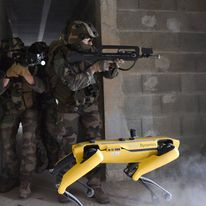
\includegraphics[width=0.3\textwidth]{r4.jpg}}
\subfigure[測試 - 軍事新聞]{
\label{Fig.sub.3}
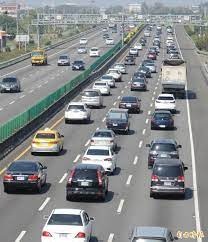
\includegraphics[width=0.3\textwidth]{r6.jpg}}
\subfigure[測試  - 新聞]{
\label{Fig.sub.4}
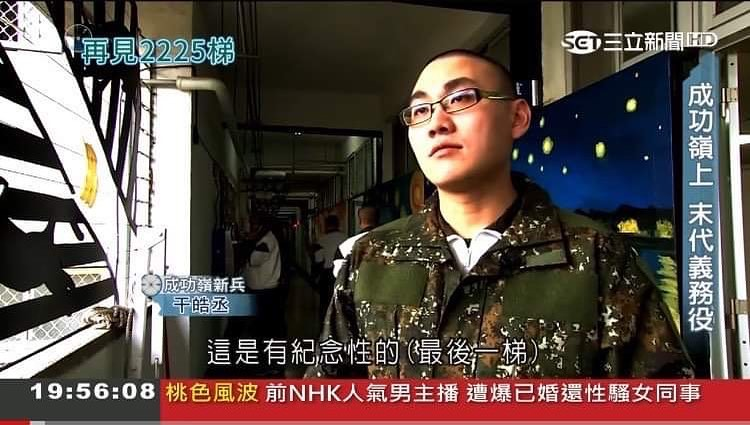
\includegraphics[width=0.3\textwidth]{r2.jpg}}
\subfigure[測試 - 自有照片]{
\label{Fig.sub.5}
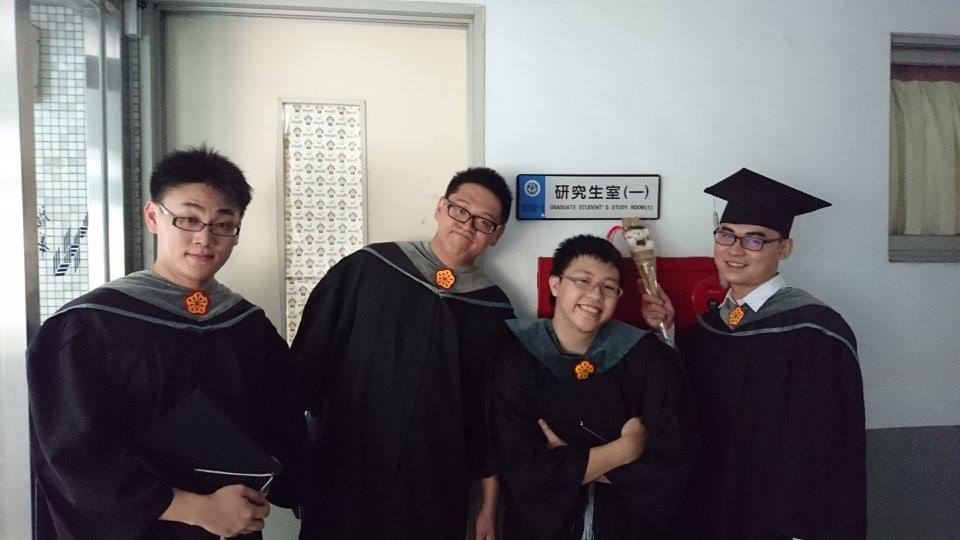
\includegraphics[width=0.3\textwidth]{r3.jpg}}
\subfigure[測試 - 新聞]{
\label{Fig.sub.6}
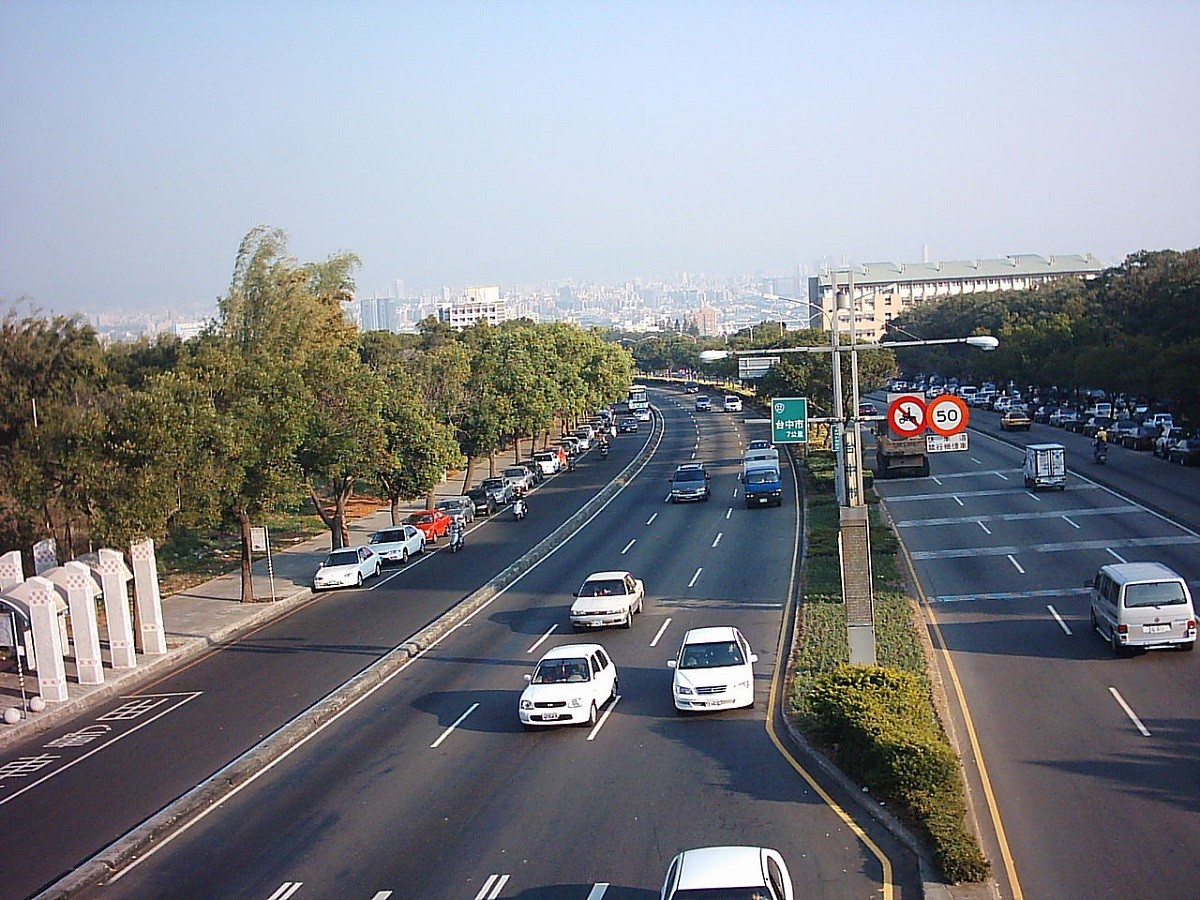
\includegraphics[width=0.3\textwidth]{r5.jpg}}
\subfigure[測試 - 新聞]{
\label{Fig.sub.7}
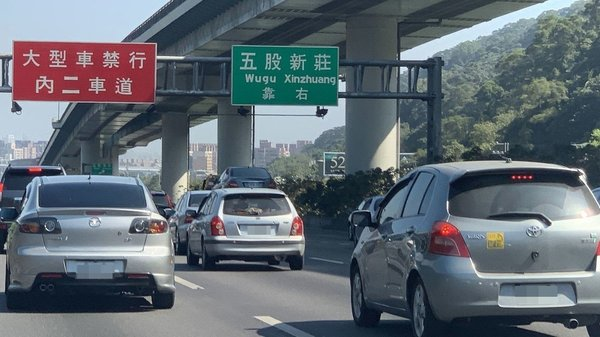
\includegraphics[width=0.3\textwidth]{r7.jpg}}
\subfigure[測試 - 官方]{
\label{Fig.sub.8}

\includegraphics[width=0.3\textwidth]{r8.jpg}}
\subfigure[測試 - 官方]{
\label{Fig.sub.9}
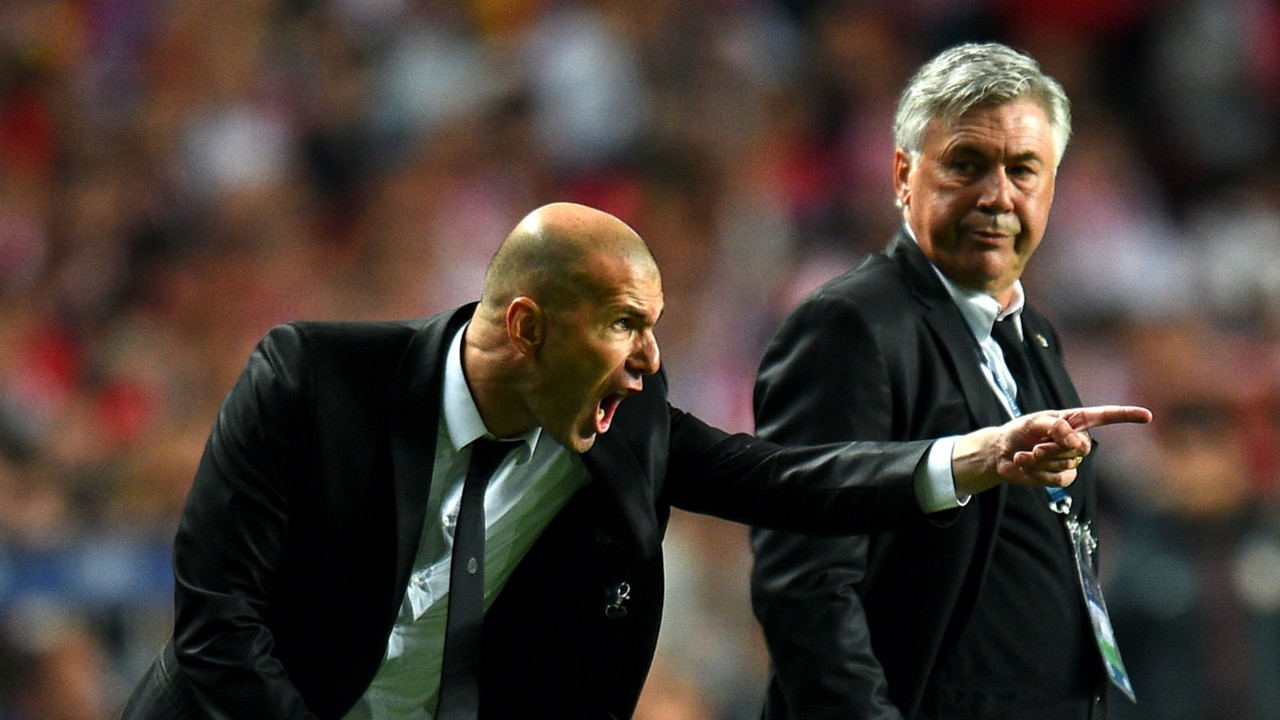
\includegraphics[width=0.3\textwidth]{r9.jpg}}
\caption{最終自有測試資料集}
\label{Fig.main}
\end{figure}

\newpage


在此列出將第一輪測試的 yolov5s.pt 與 yolov5m.pt 的結果與原始資料進行比較。可以在過程中看到差異。

\begin{figure}[H]
\centering  %圖片全局居中
\subfigure[原始相片]{
\label{Fig.sub.1}
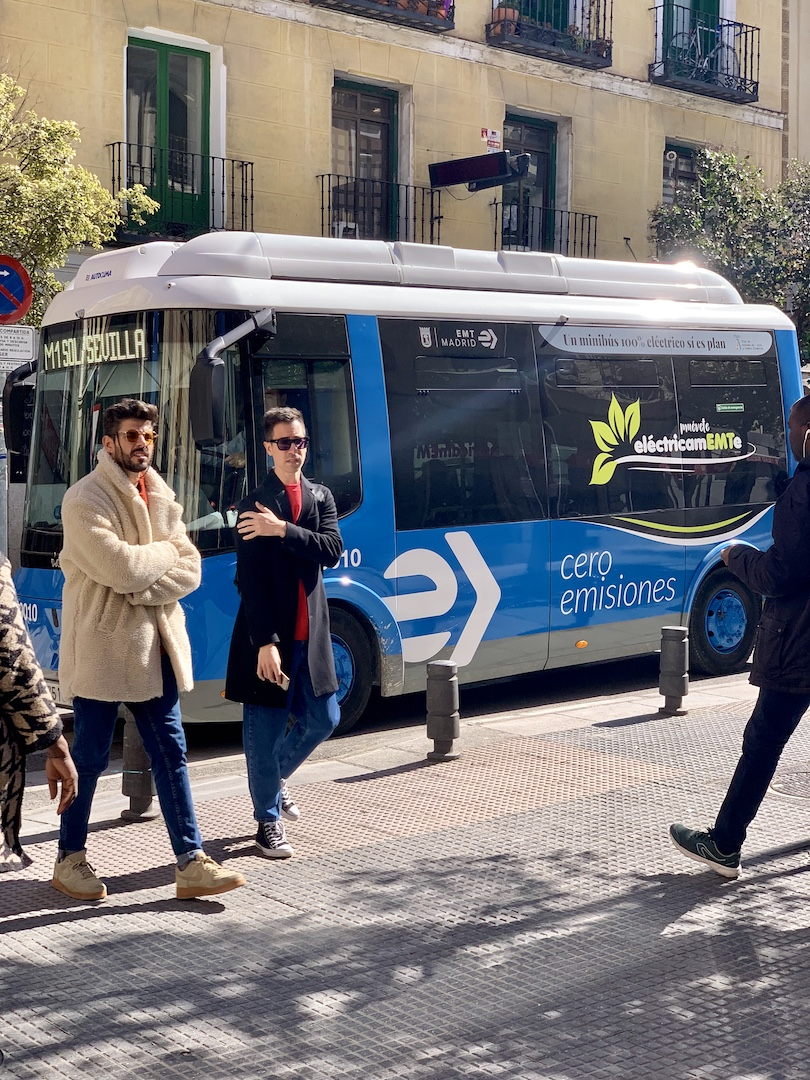
\includegraphics[width=0.3\textwidth]{r1.jpg}}
\subfigure[yolov5s.pt]{
\label{Fig.sub.2}
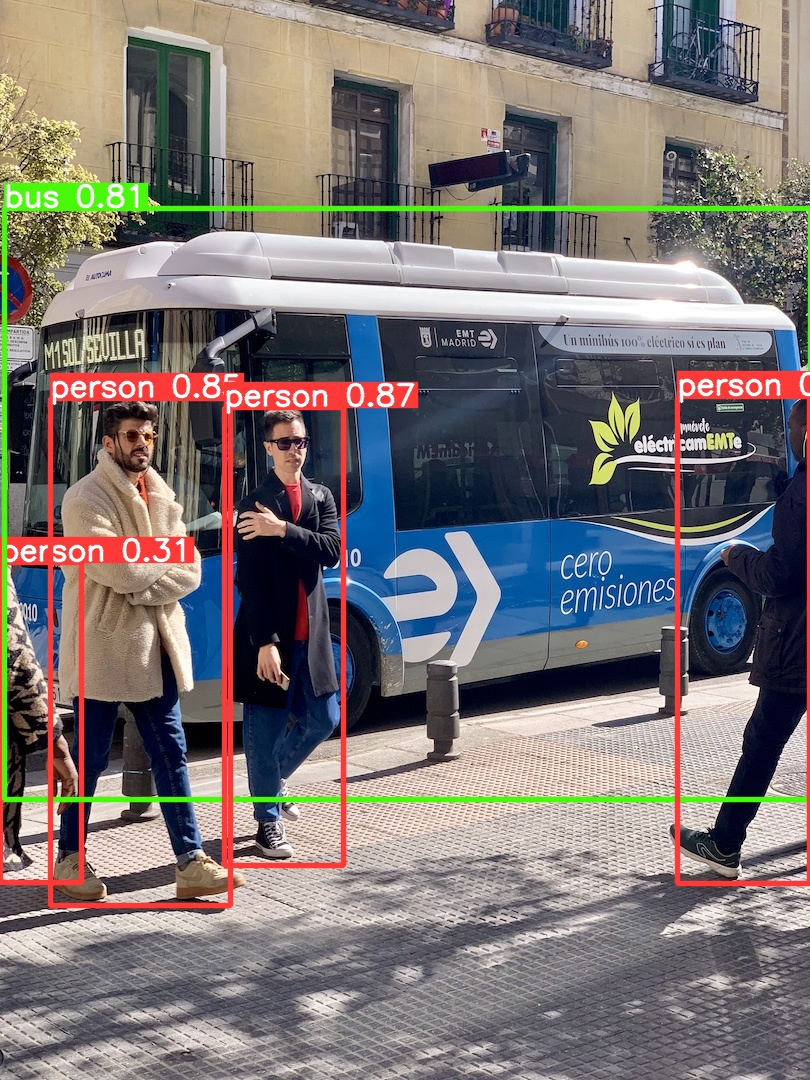
\includegraphics[width=0.3\textwidth]{o61.jpg}}
\subfigure[yolov5m.pt]{
\label{Fig.sub.3}
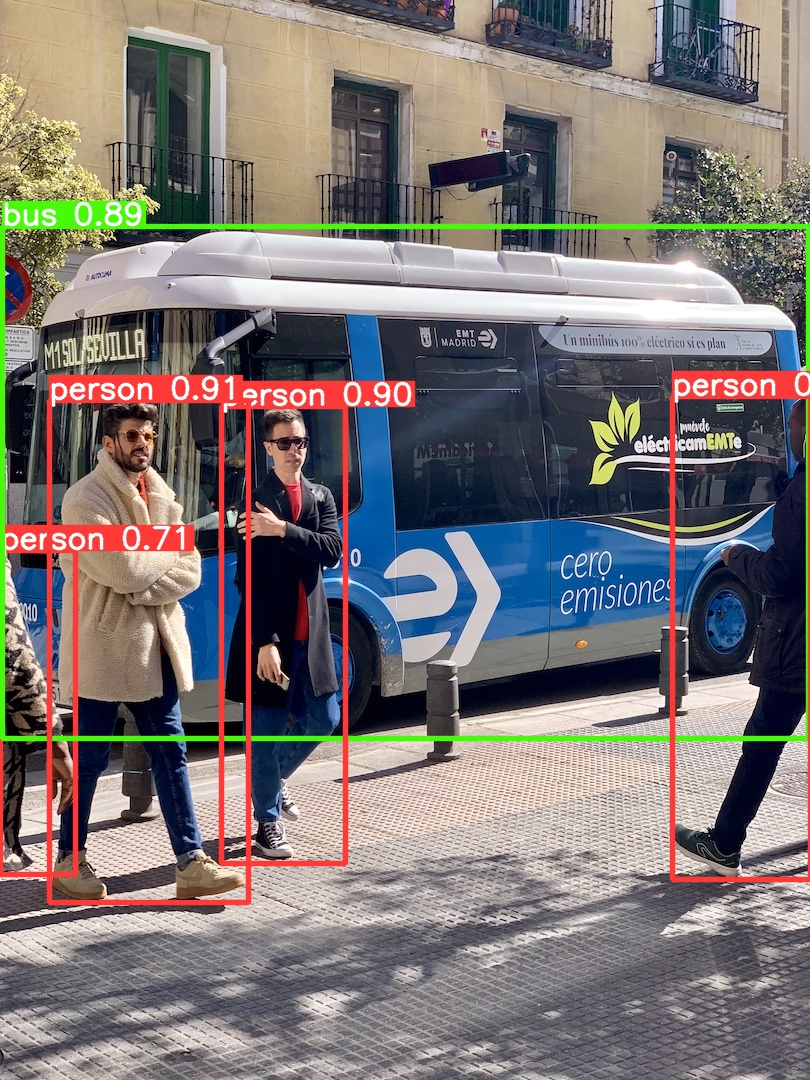
\includegraphics[width=0.3\textwidth]{o71.jpg}}
\caption{測試 1 - 官方}
\label{Fig.main}
\end{figure}

\begin{figure}[H]
\centering  %圖片全局居中
\subfigure[原始相片]{
\label{Fig.sub.1}
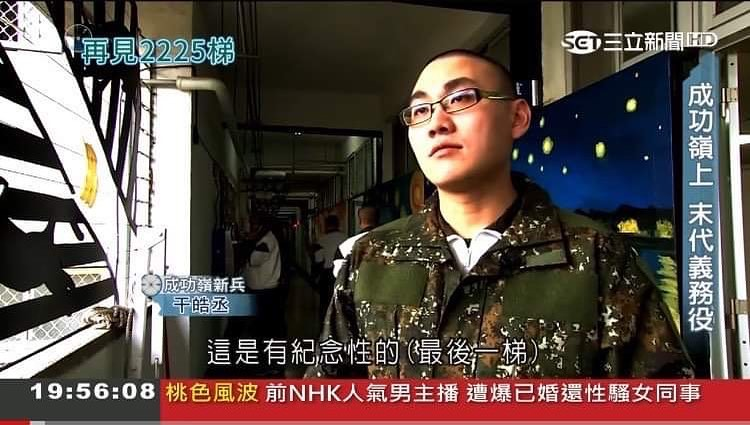
\includegraphics[width=0.9\textwidth]{r2.jpg}}
\subfigure[yolov5s.pt]{
\label{Fig.sub.2}
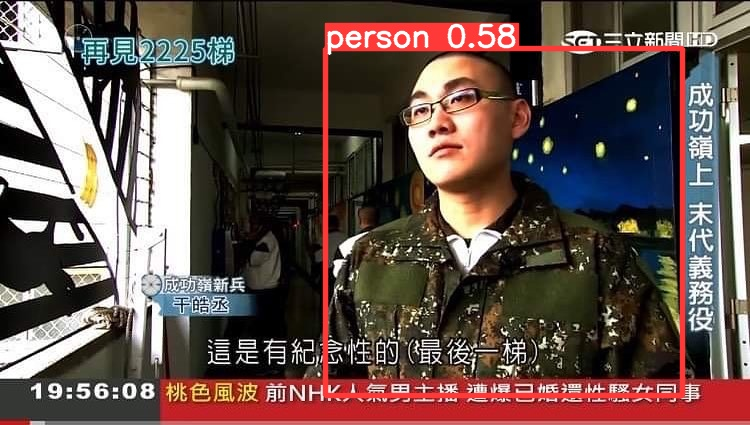
\includegraphics[width=0.4\textwidth]{o62.jpg}}
\subfigure[yolov5m.pt]{
\label{Fig.sub.3}
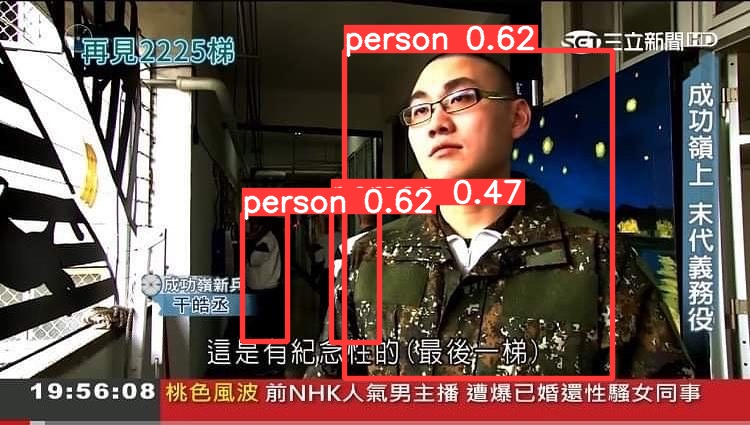
\includegraphics[width=0.4\textwidth]{o73.jpg}}
\caption{測試 2 - 新聞採訪}
\label{Fig.main}
\end{figure}

\begin{figure}[H]
\centering  %圖片全局居中
\subfigure[原始相片]{
\label{Fig.sub.1}
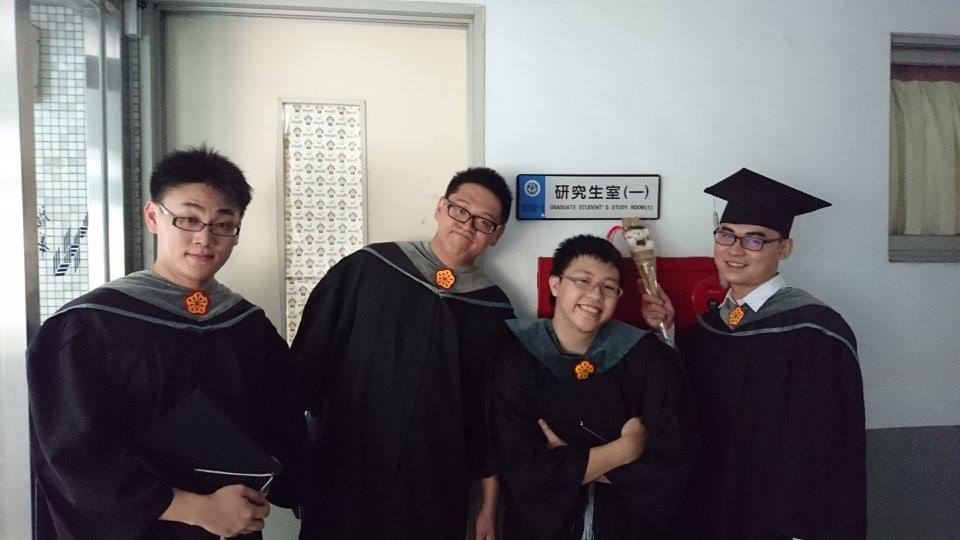
\includegraphics[width=0.3\textwidth]{r3.jpg}}
\subfigure[yolov5s.pt]{
\label{Fig.sub.2}
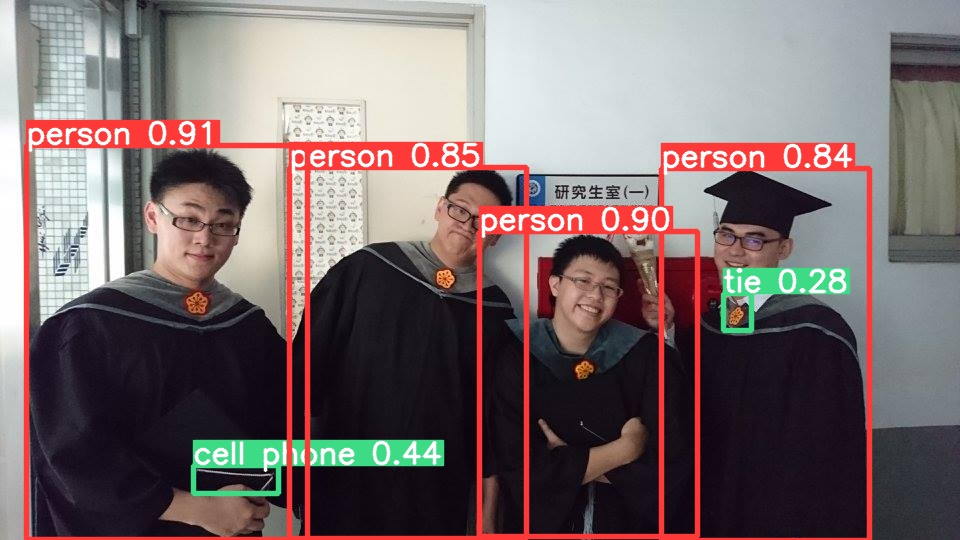
\includegraphics[width=0.3\textwidth]{o63.jpg}}
\subfigure[yolov5m.pt]{
\label{Fig.sub.3}
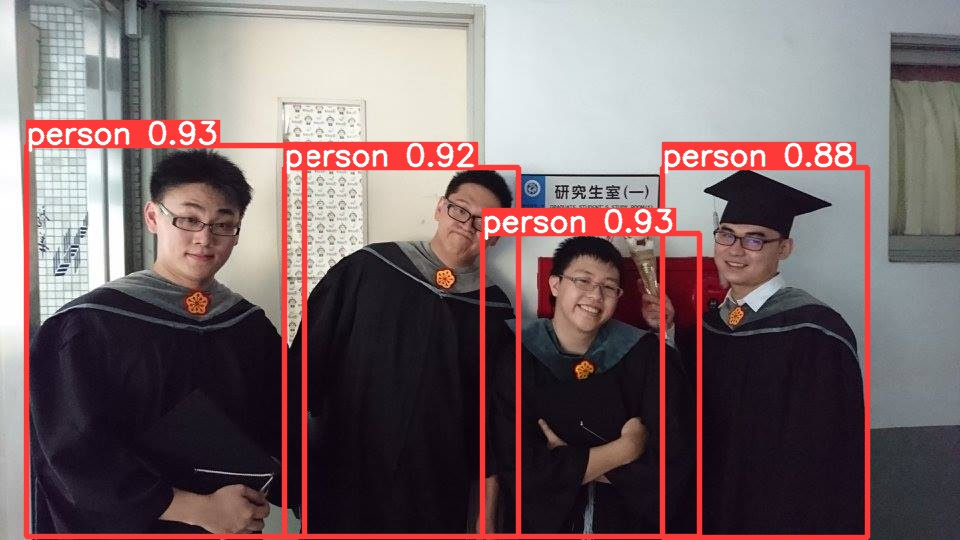
\includegraphics[width=0.3\textwidth]{o74.jpg}}
\caption{測試 3 - 自有照片}
\label{Fig.main}
\end{figure}

\begin{figure}[H]
\centering  %圖片全局居中
\subfigure[原始相片]{
\label{Fig.sub.1}
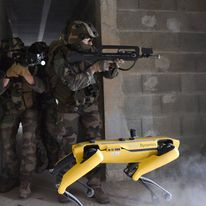
\includegraphics[width=0.3\textwidth]{r4.jpg}}
\subfigure[yolov5s.pt]{
\label{Fig.sub.2}
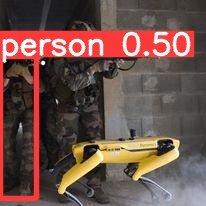
\includegraphics[width=0.3\textwidth]{o64.jpg}}
\subfigure[yolov5m.pt]{
\label{Fig.sub.3}
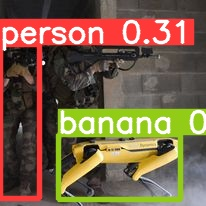
\includegraphics[width=0.3\textwidth]{o75.jpg}}
\caption{測試 4 - 軍事新聞}
\label{Fig.main}
\end{figure}

\begin{figure}[H]
\centering  %圖片全局居中
\subfigure[原始相片]{
\label{Fig.sub.1}
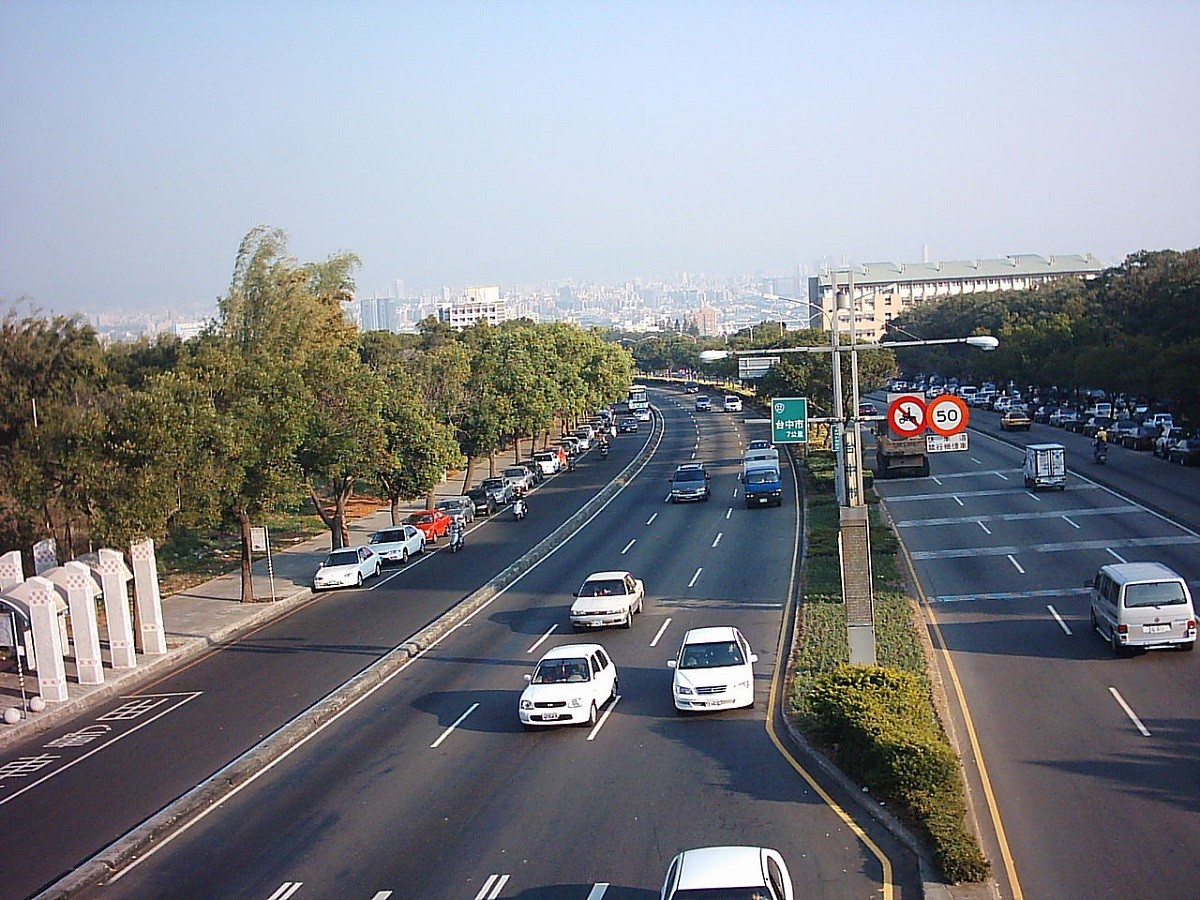
\includegraphics[width=0.4\textwidth]{r5.jpg}}
\subfigure[yolov5m.pt]{
\label{Fig.sub.2}
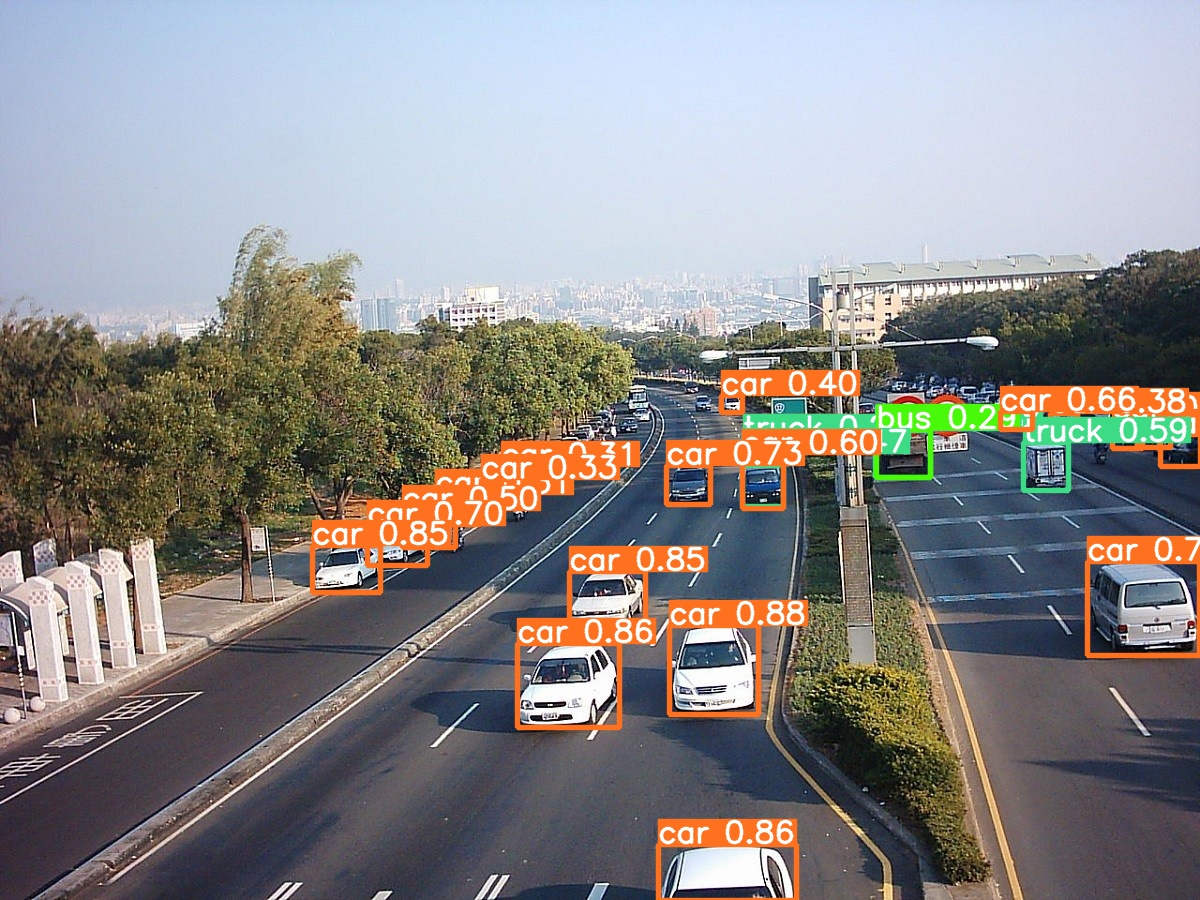
\includegraphics[width=0.4\textwidth]{o76.jpg}}
\caption{測試 5 - 新聞}
\label{Fig.main}
\end{figure}


\begin{figure}[H]
\centering  %圖片全局居中
\subfigure[原始相片]{
\label{Fig.sub.1}
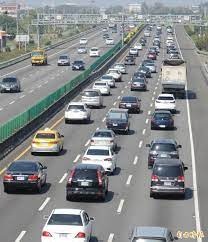
\includegraphics[width=0.3\textwidth]{r6.jpg}}
\subfigure[yolov5s.pt]{
\label{Fig.sub.2}
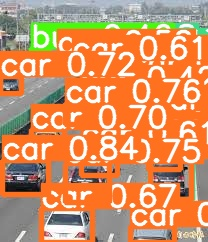
\includegraphics[width=0.3\textwidth]{o65.jpg}}
\subfigure[yolov5m.pt]{
\label{Fig.sub.3}
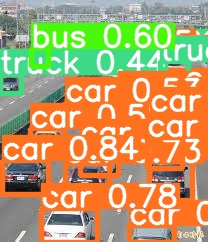
\includegraphics[width=0.3\textwidth]{o77.jpg}}
\caption{測試 6 - 新聞}
\label{Fig.main}
\end{figure}

\begin{figure}[H]
\centering  %圖片全局居中
\subfigure[原始相片]{
\label{Fig.sub.1}
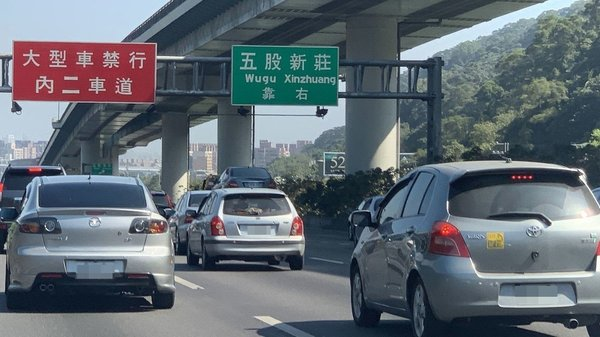
\includegraphics[width=0.4\textwidth]{r7.jpg}}
\subfigure[yolov5m.pt]{
\label{Fig.sub.2}
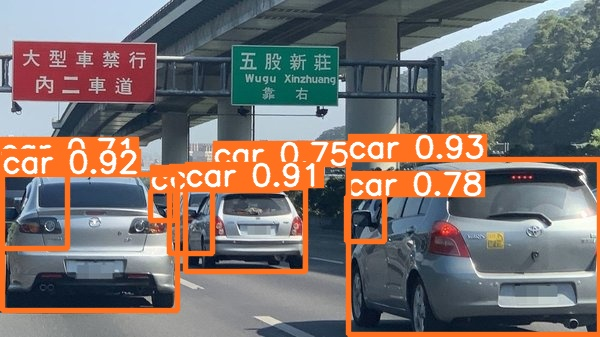
\includegraphics[width=0.4\textwidth]{o78.jpg}}
\caption{測試 7 - 新聞}
\label{Fig.main}
\end{figure}

\begin{figure}[H]
\centering  %圖片全局居中
\subfigure[原始相片]{
\label{Fig.sub.1}

\includegraphics[width=0.4\textwidth]{r8.jpg}}
\subfigure[yolov5m.pt]{
\label{Fig.sub.2}
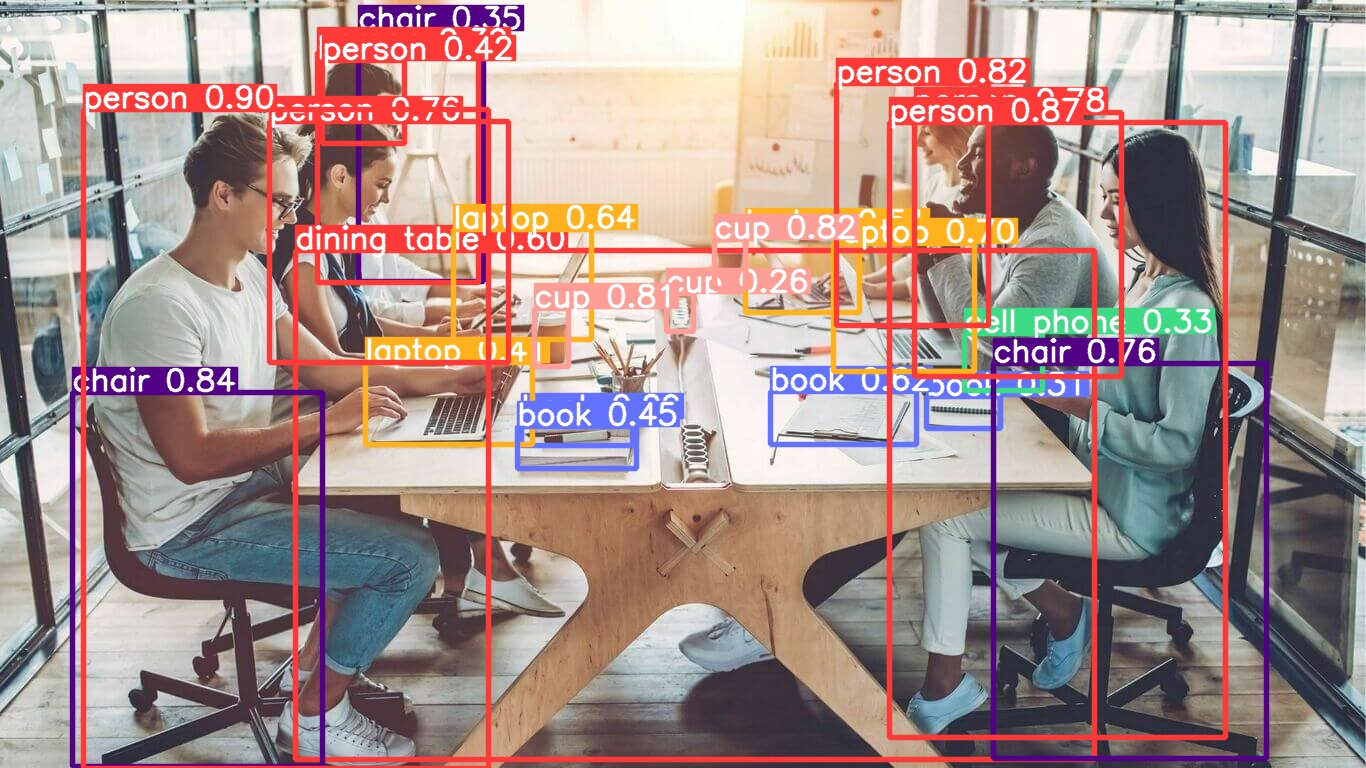
\includegraphics[width=0.4\textwidth]{o79.jpg}}
\caption{測試 8 - 官方}
\label{Fig.main}
\end{figure}

\begin{figure}[H]
\centering  %圖片全局居中
\subfigure[原始相片]{
\label{Fig.sub.1}
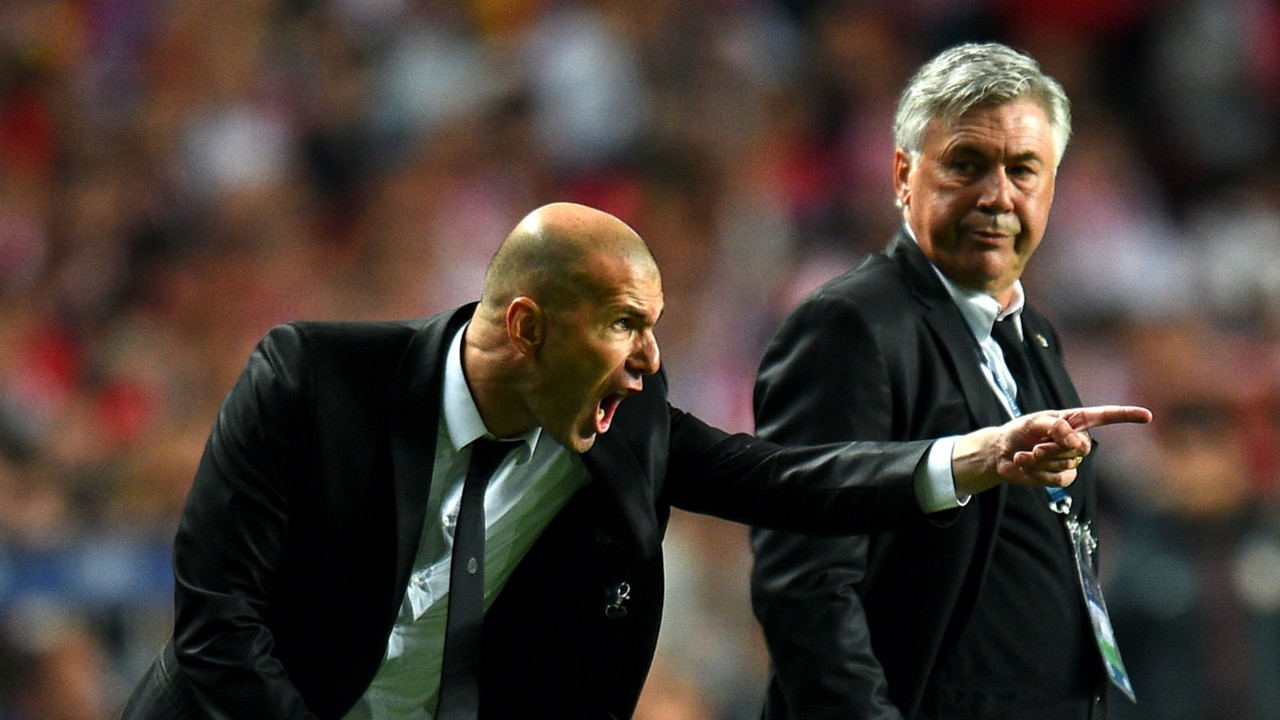
\includegraphics[width=0.3\textwidth]{r9.jpg}}
\subfigure[yolov5s.pt]{
\label{Fig.sub.2}
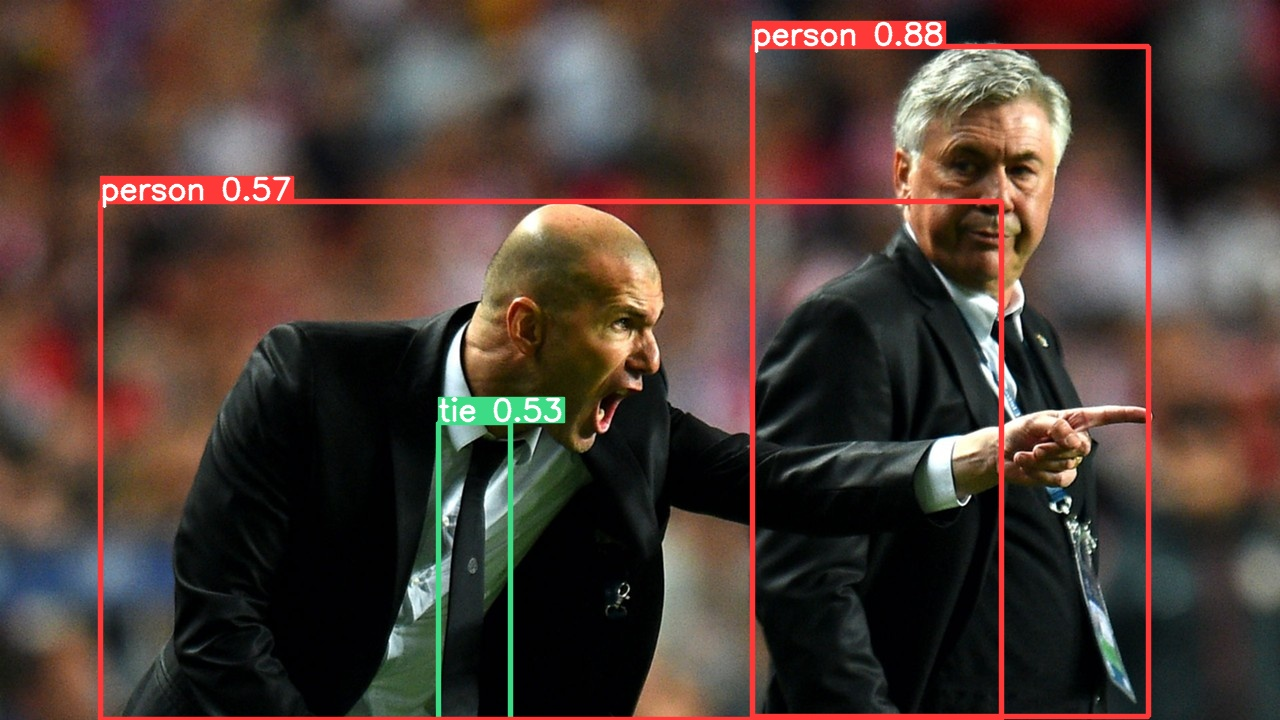
\includegraphics[width=0.3\textwidth]{o66.jpg}}
\subfigure[yolov5m.pt]{
\label{Fig.sub.3}
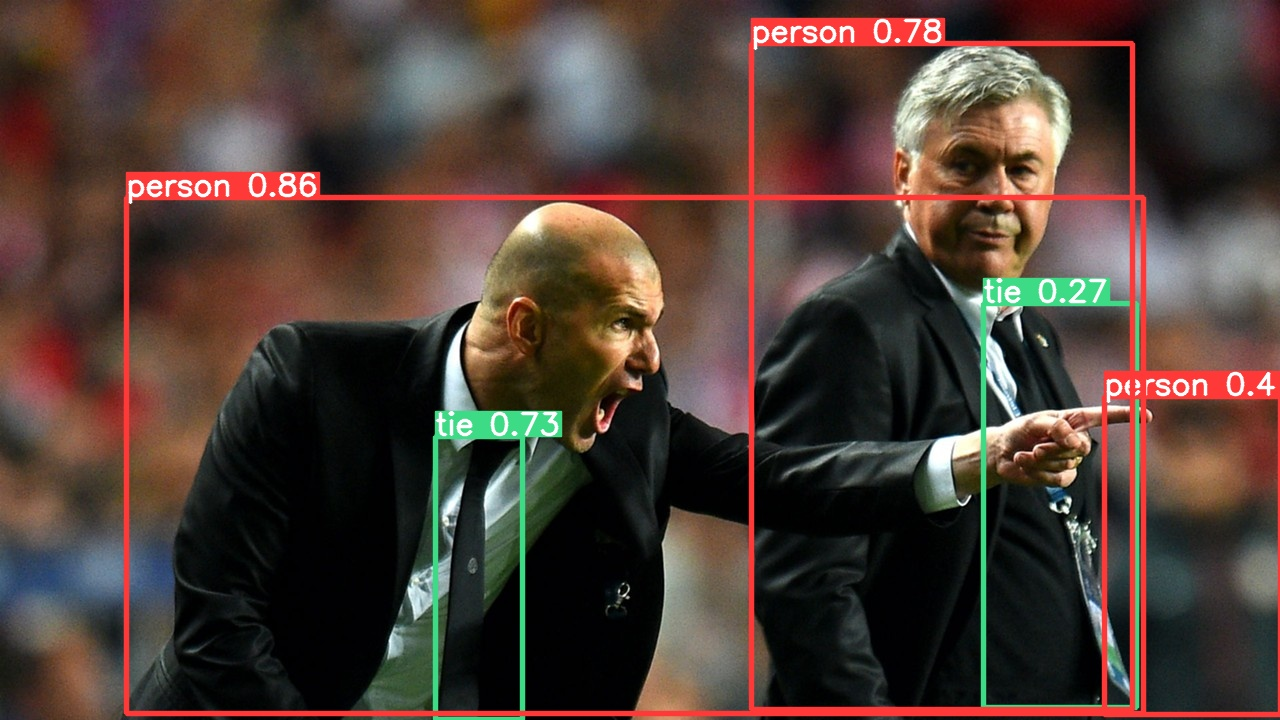
\includegraphics[width=0.3\textwidth]{o72.jpg}}
\caption{測試 9 - 官方}
\label{Fig.main}
\end{figure}


此部分為 YOLOv5 的 Pytorch 官方 Google Colab 範例結果執行後,輸出的呈現。一共分為 ext1 與 ext2 的部分。

\begin{figure}[H]
\centering 
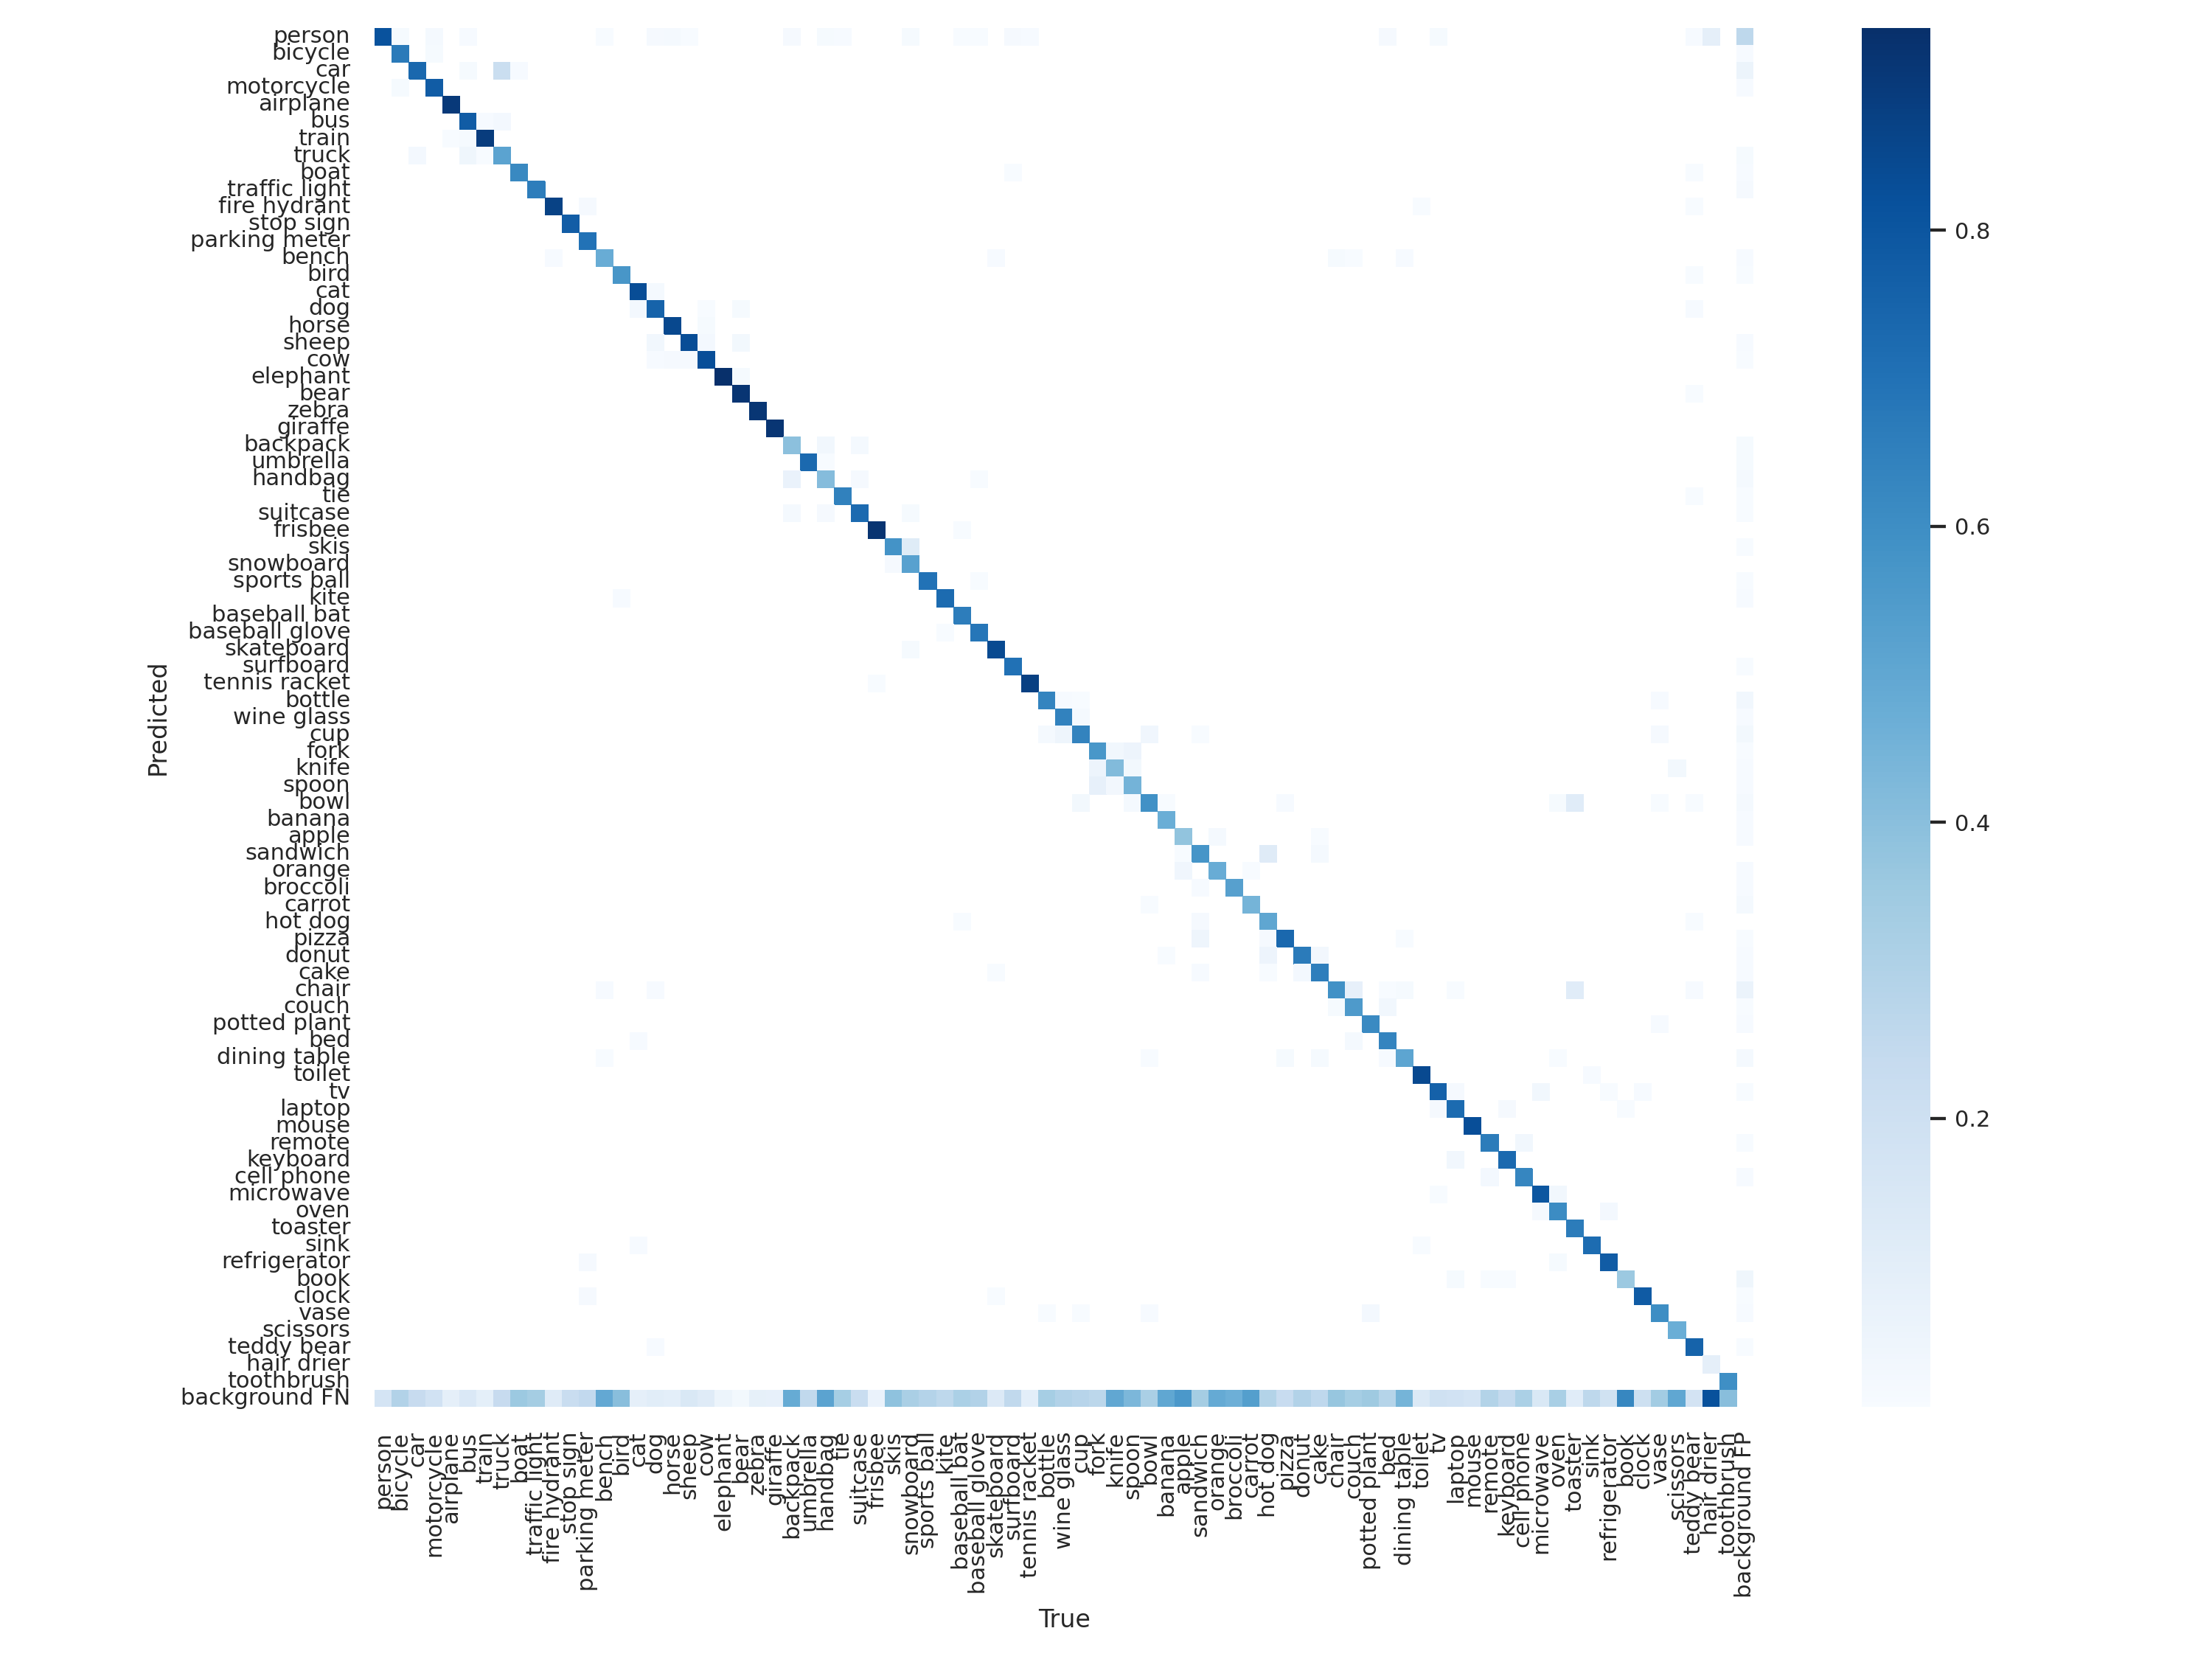
\includegraphics[width=0.90\textwidth]{ex11.png} 
\caption{ext1 - 1}
\label{Test}
\end{figure}

\begin{figure}[H]
\centering 
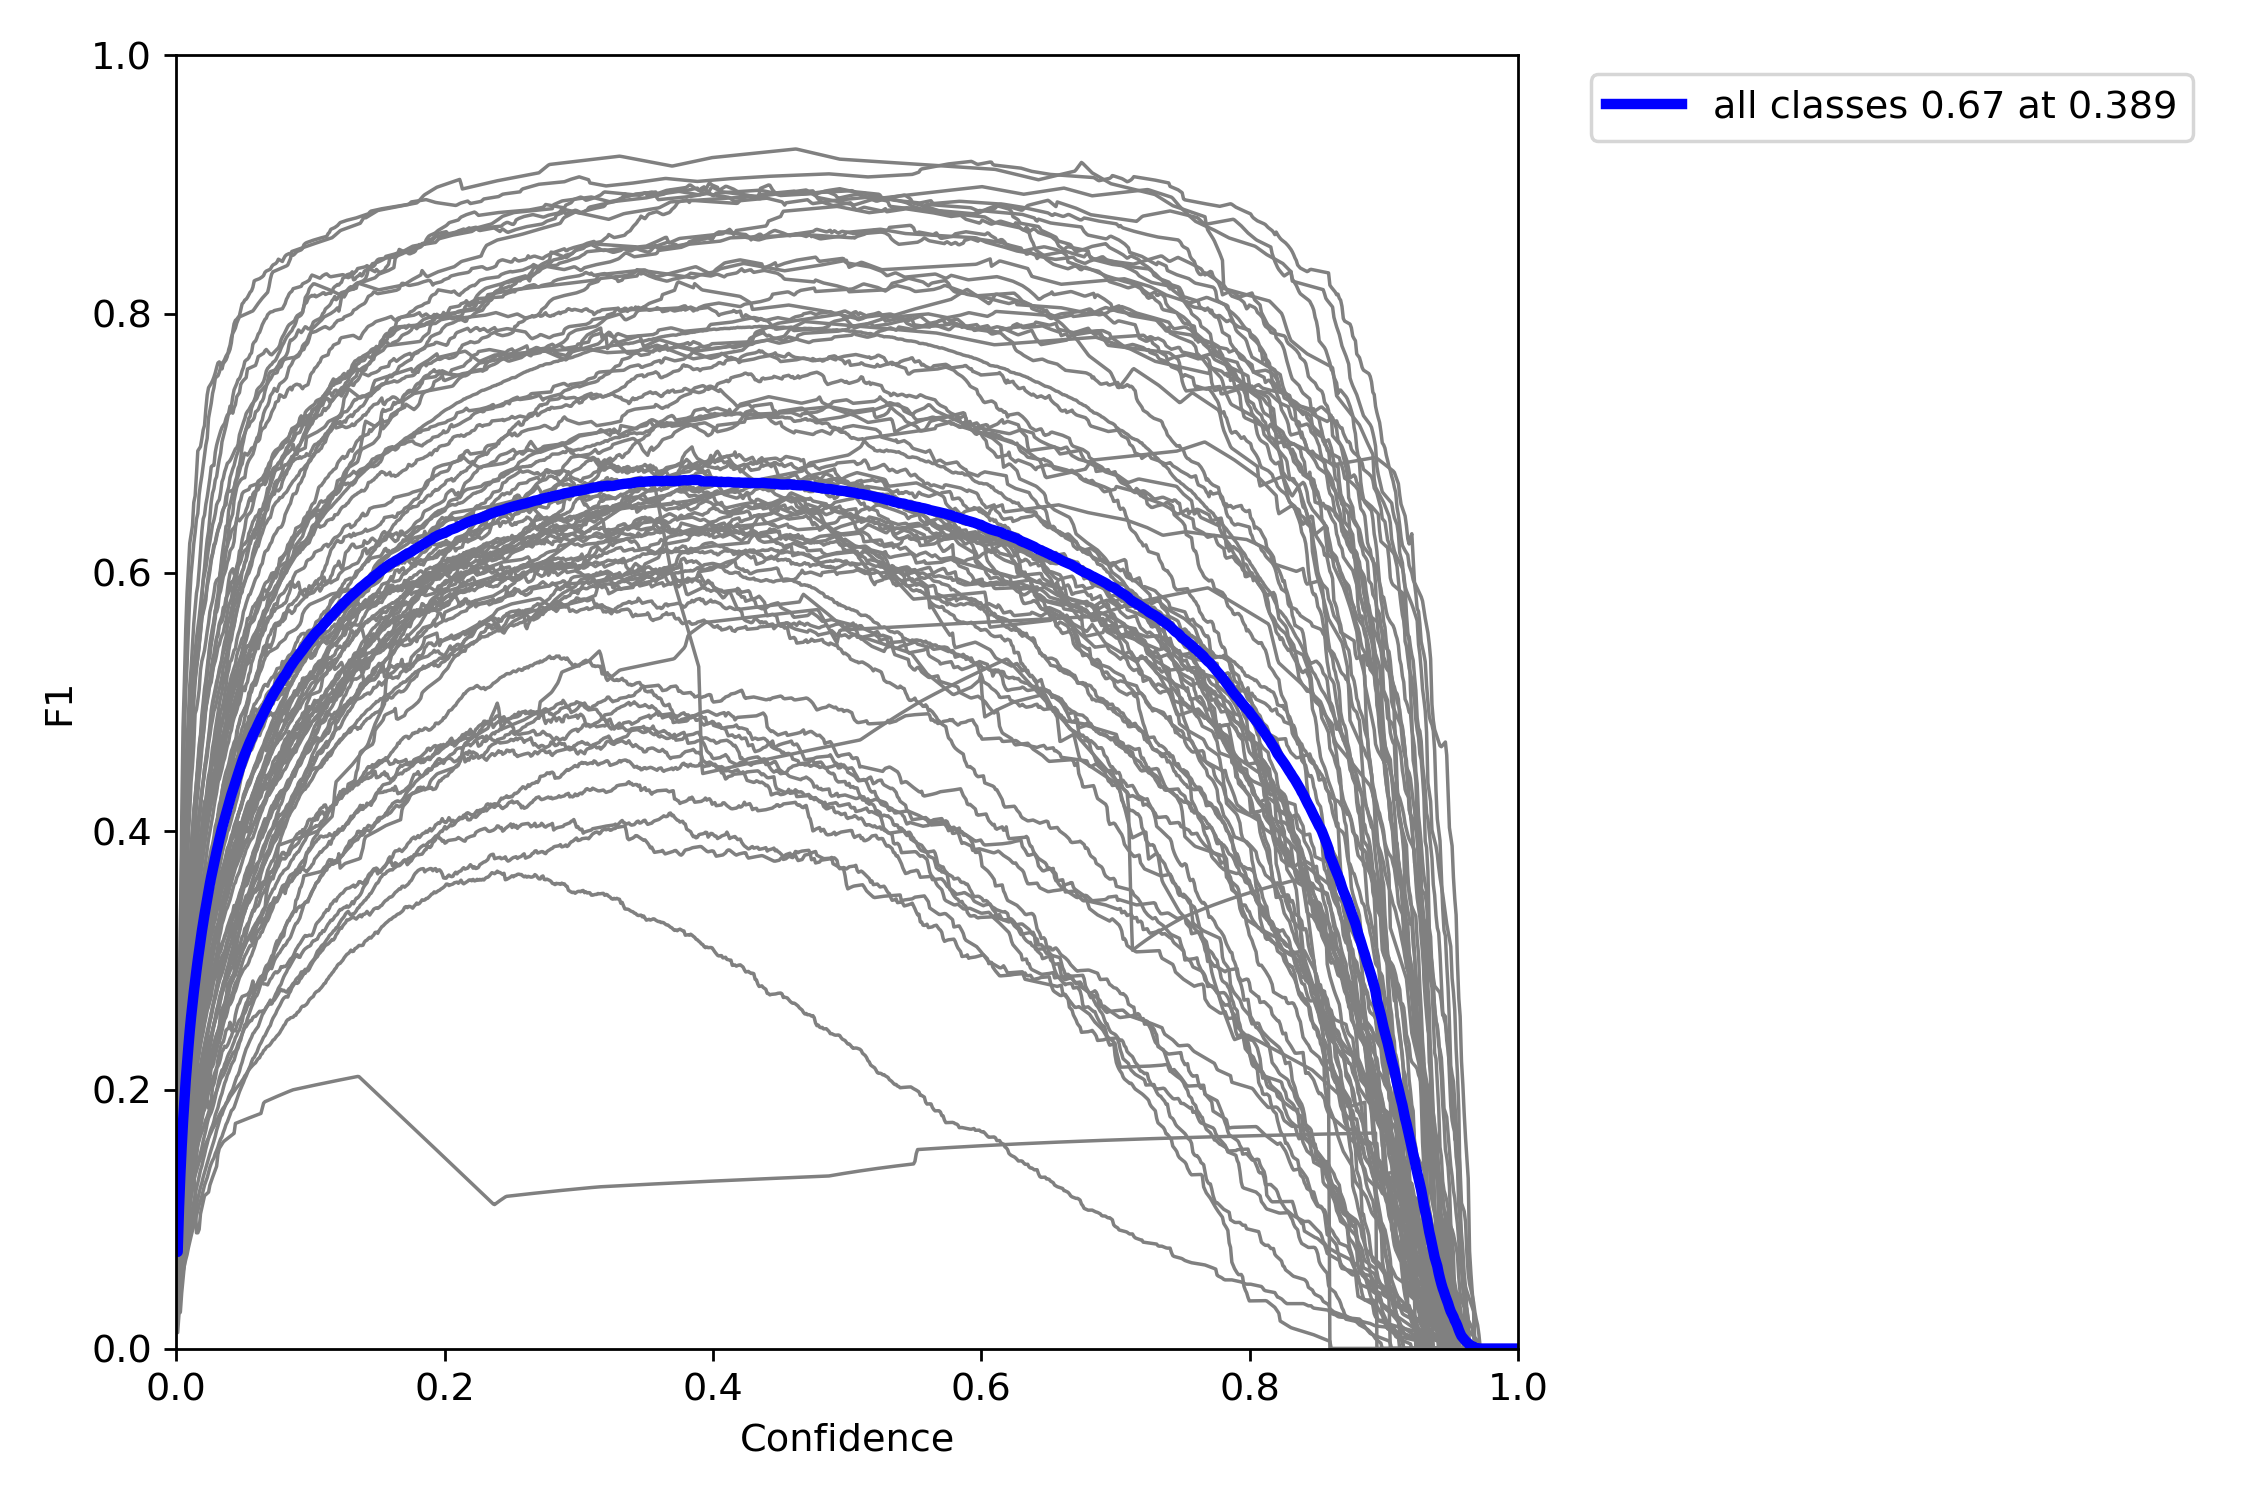
\includegraphics[width=0.90\textwidth]{ex12.png} 
\caption{ext1 - 2}
\label{Test}
\end{figure}

\begin{figure}[H]
\centering 
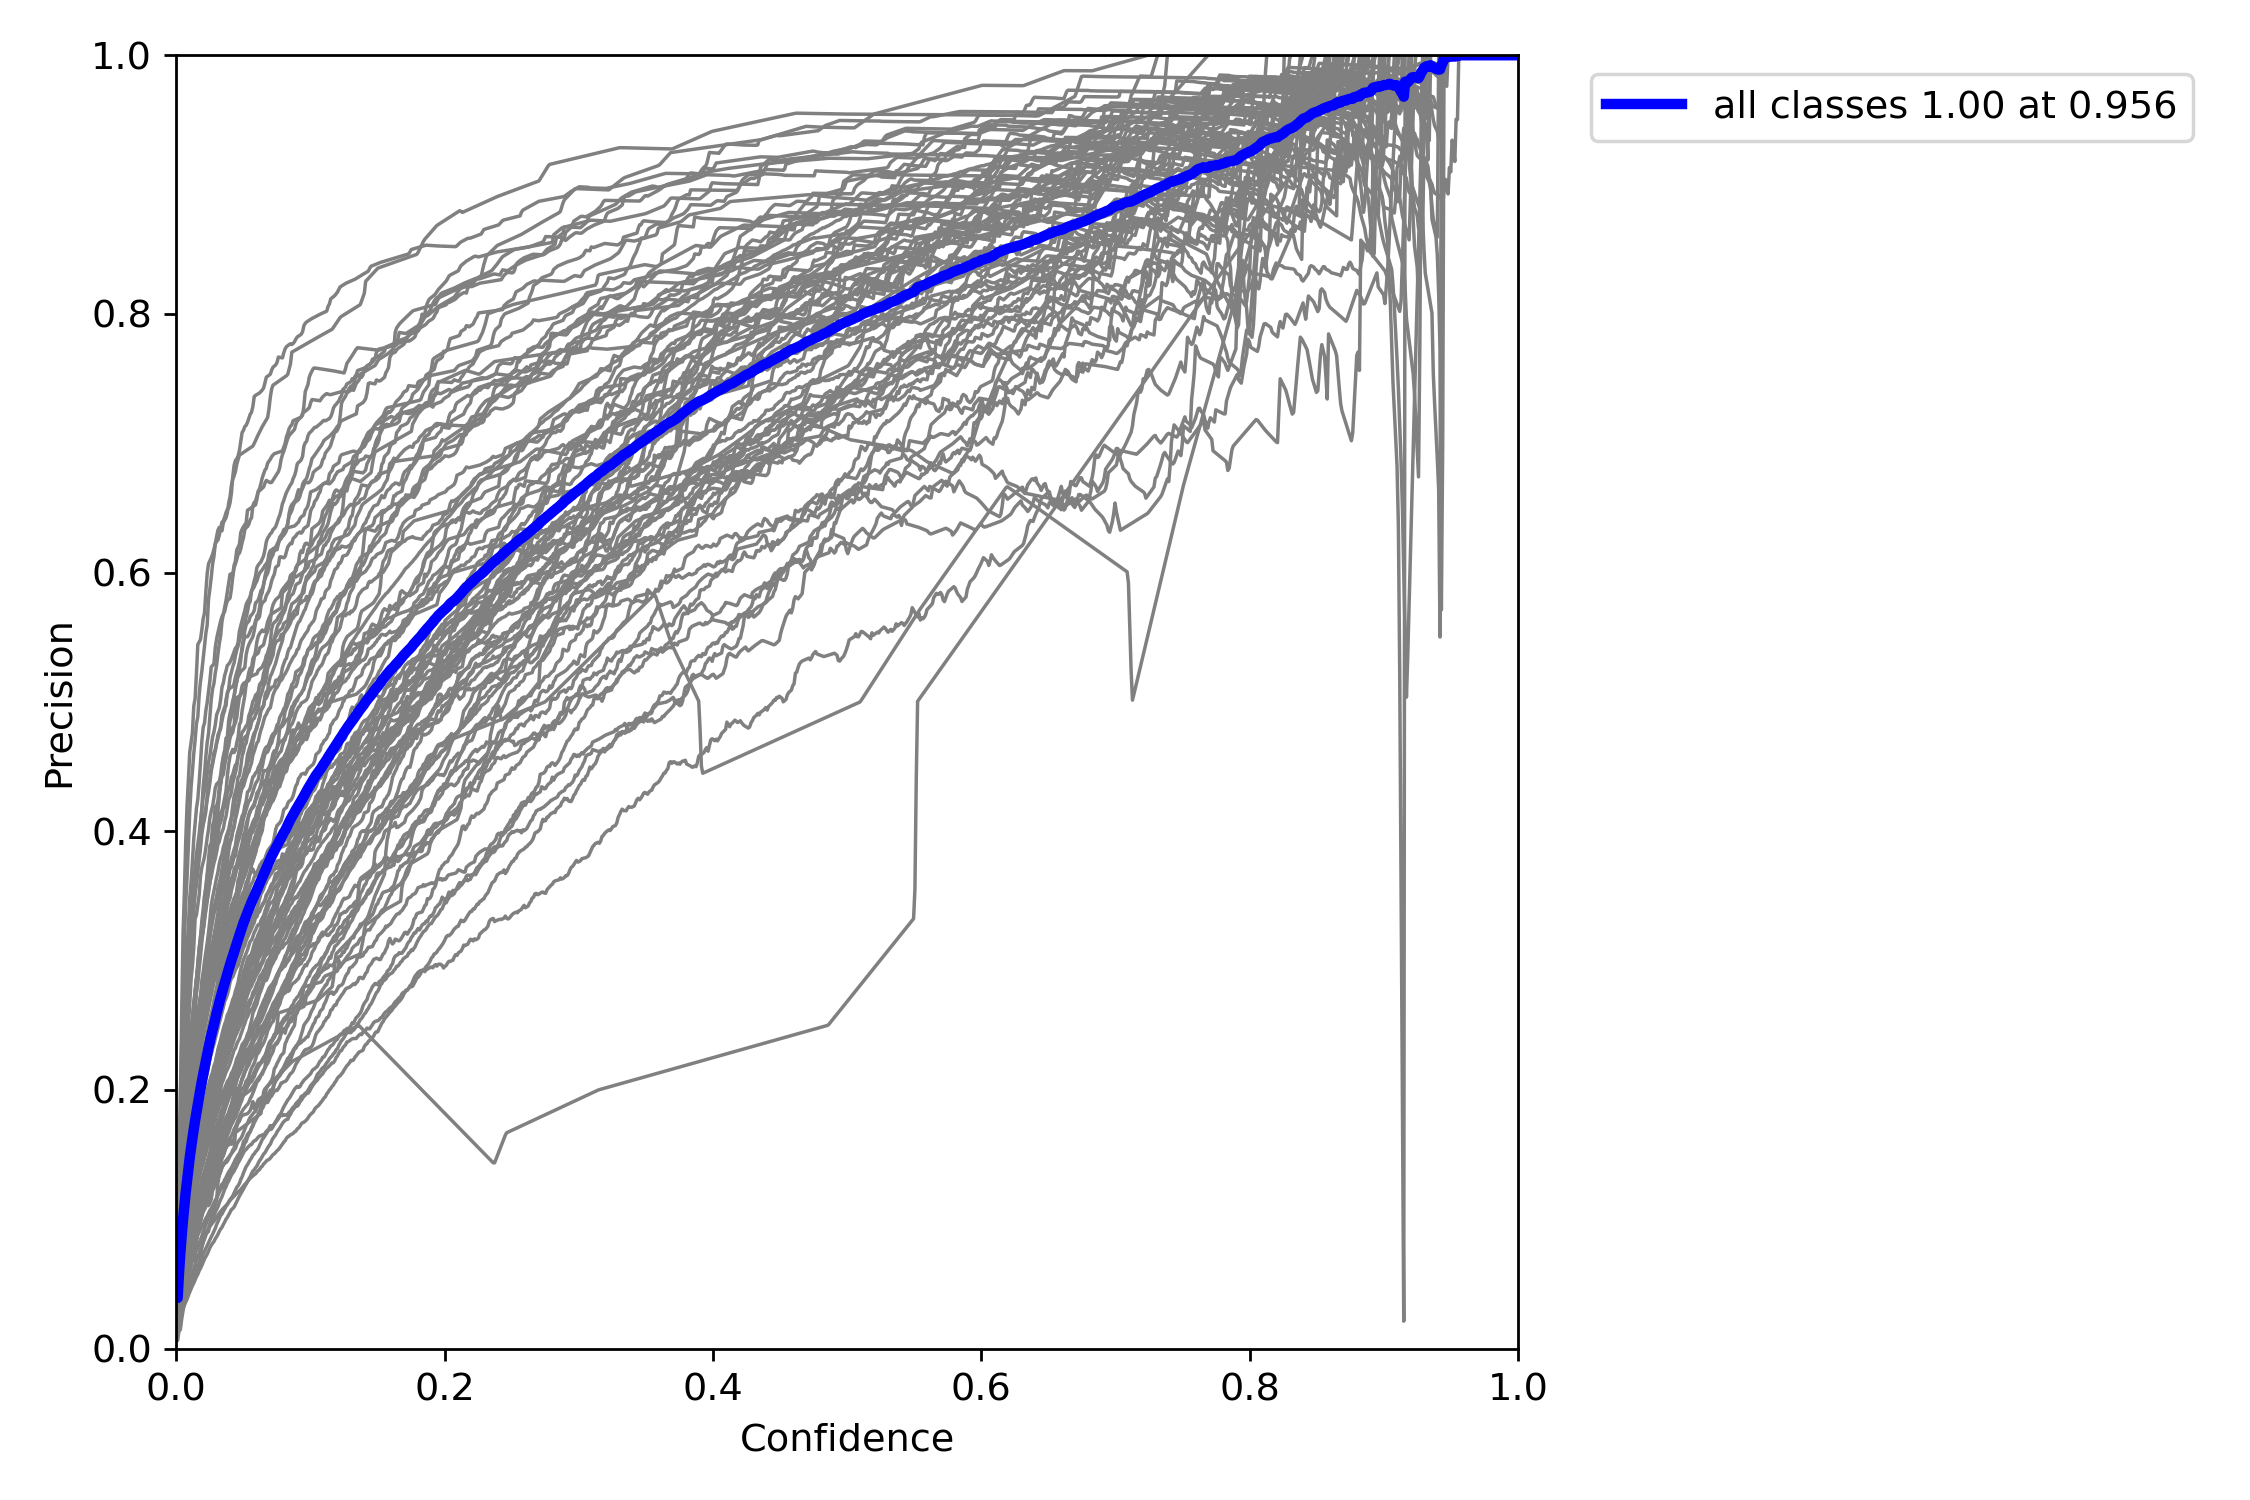
\includegraphics[width=0.90\textwidth]{ex13.png} 
\caption{ext1 - 3}
\label{Test}
\end{figure}

\begin{figure}[H]
\centering 
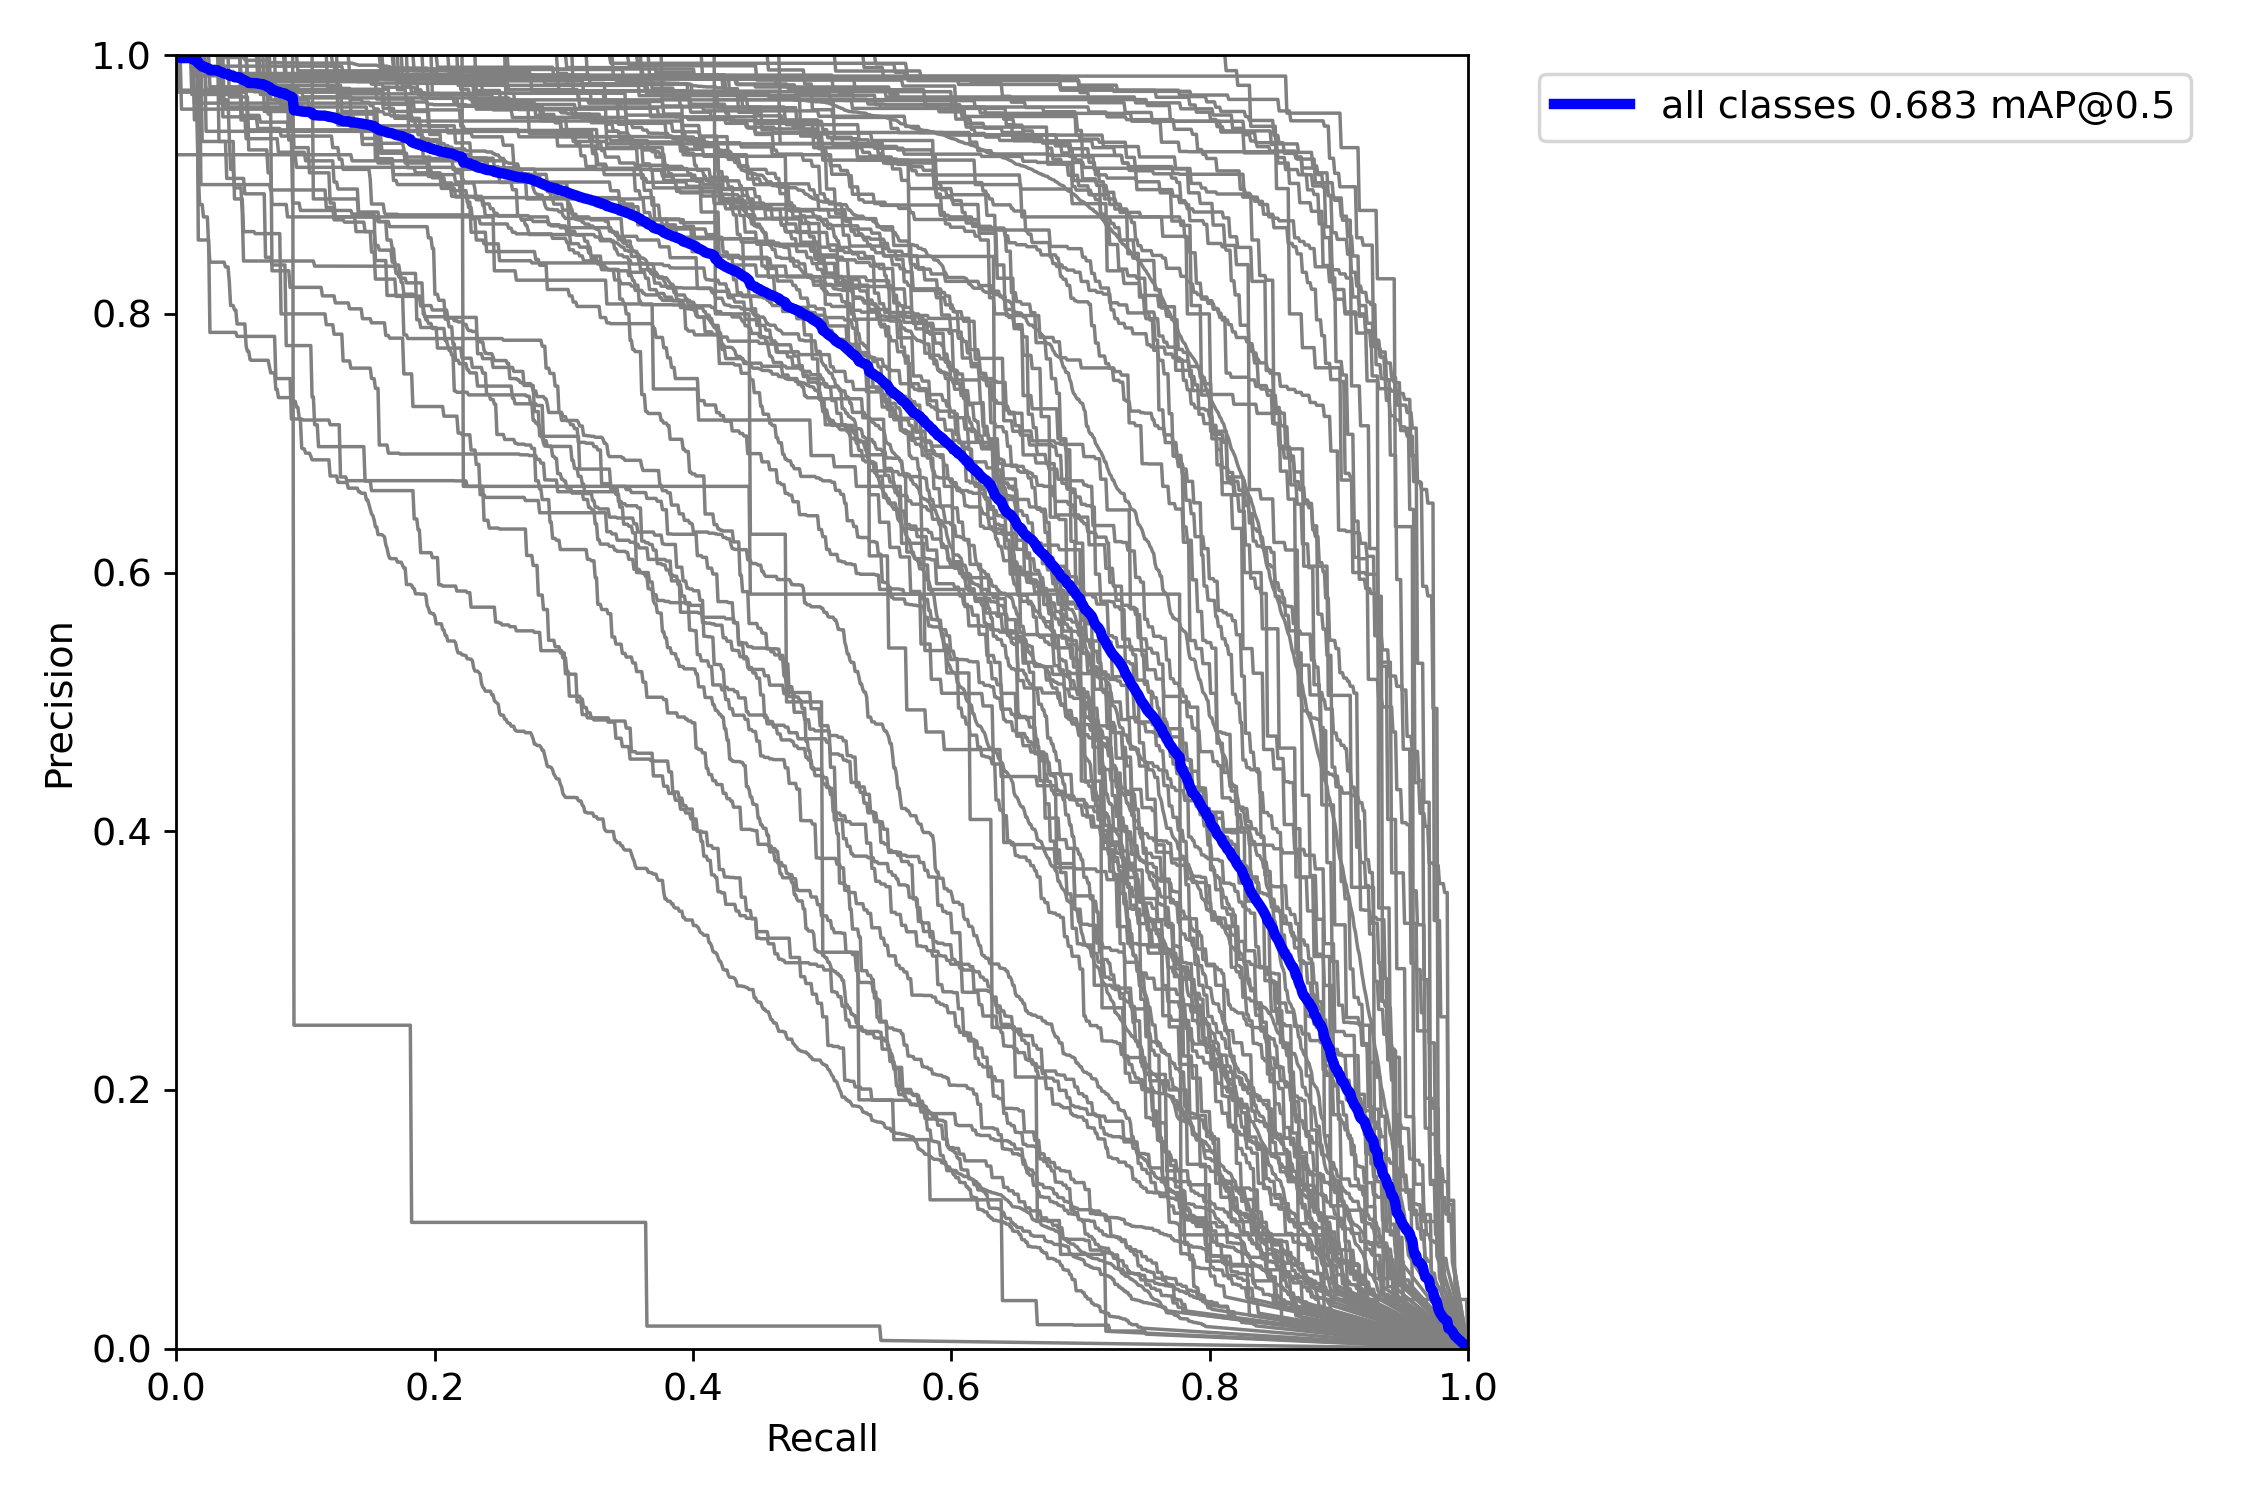
\includegraphics[width=0.90\textwidth]{ex14.png} 
\caption{ext1 - 4}
\label{Test}
\end{figure}

\begin{figure}[H]
\centering 
\includegraphics[width=0.90\textwidth]{ex15.png} 
\caption{ext1 - 5}
\label{Test}
\end{figure}

\begin{figure}[H]
\centering 
\includegraphics[width=0.90\textwidth]{ex16.jpg} 
\caption{ext1 - 6}
\label{Test}
\end{figure}

\begin{figure}[H]
\centering 
\includegraphics[width=0.90\textwidth]{ex17.jpg} 
\caption{ext1 - 7}
\label{Test}
\end{figure}

\begin{figure}[H]
\centering 
\includegraphics[width=0.90\textwidth]{ex18.jpg} 
\caption{ext1 - 8}
\label{Test}
\end{figure}

\begin{figure}[H]
\centering 
\includegraphics[width=0.90\textwidth]{ex19.jpg} 
\caption{ext1 - 9}
\label{Test}
\end{figure}

\begin{figure}[H]
\centering 
\includegraphics[width=0.90\textwidth]{ex110.jpg} 
\caption{ext1 - 9}
\label{Test}
\end{figure}

\begin{figure}[H]
\centering 
\includegraphics[width=0.90\textwidth]{ex111.jpg} 
\caption{ext1 - 9}
\label{Test}
\end{figure}

\begin{figure}[H]
\centering 
\includegraphics[width=0.90\textwidth]{ex21.png} 
\caption{ext2 - 1}
\label{Test}
\end{figure}

\begin{figure}[H]
\centering 
\includegraphics[width=0.90\textwidth]{ex22.jpg} 
\caption{ext2 - 2}
\label{Test}
\end{figure}

\begin{figure}[H]
\centering 
\includegraphics[width=0.90\textwidth]{ex23.jpg} 
\caption{ext2 - 3}
\label{Test}
\end{figure}

\begin{figure}[H]
\centering 
\includegraphics[width=0.90\textwidth]{ex24.jpg} 
\caption{ext2 - 4}
\label{Test}
\end{figure}

\begin{figure}[H]
\centering 
\includegraphics[width=0.90\textwidth]{ex25.jpg} 
\caption{ext2 - 5}
\label{Test}
\end{figure}

\begin{figure}[H]
\centering 
\includegraphics[width=0.90\textwidth]{ex26.jpg} 
\caption{ext2 - 6}
\label{Test}
\end{figure}

\begin{figure}[H]
\centering 
\includegraphics[width=0.90\textwidth]{ex27.jpg} 
\caption{ext2 - 7}
\label{Test}
\end{figure}
%\section{附錄}

% 數學意義說明

% $$\min \limits_{G}\max \limits_{D}{V_I(D,\ G)=V(D,G)-\lambda L_I(G,Q)}$$

%	\begin{lstlisting}[language={python}]

%	\end{lstlisting}

%\begin{enumerate}
%\item Y
%\item A
%\end{enumerate}

% \newpage

\clearpage

\end{document}